\documentclass[12pt]{article}
% load packages
\usepackage{amssymb,amsmath,amsfonts,geometry,graphicx,color,setspace,natbib,hyperref}
\usepackage{kpfonts}
%\usepackage{tgpagella}
%\usepackage{mathpazo}
%\usepackage[osf,sc]{mathpazo}
%\usepackage{lipsum}
%\usepackage{newpxtext,newpxmath}
\usepackage{booktabs}
\usepackage[flushleft]{threeparttable}
%\usepackage{subcaption}
\usepackage{siunitx}
%\usepackage[capposition=top]{floatrow}
\usepackage[table,xcdraw]{xcolor}
\usepackage{placeins}
\usepackage{lineno}


\usepackage{natbib}

\usepackage{tabularx} % in the preamble
\usepackage{dsfont}
\usepackage{wrapfig}
\usepackage[nameinlink,capitalise]{cleveref}
\newcommand{\crefrangeconjunction}{--}

\usepackage[tableposition=top, labelfont=bf]{caption}
\DeclareCaptionFont{xipt}{\bfseries\fontfamily{qag}\selectfont}
\usepackage[font=xipt, labelfont=bf, textfont=bf]{caption}
\setlength{\abovecaptionskip}{0.2cm}


%\renewcommand{\thesubfigure}{\Alph{subfigure}}
%\captionsetup[subfigure]{font={bf,large}, labelformat=simple, skip=1pt, singlelinecheck=false}

%\sisetup{
%  per-mode=symbol,
%  group-separator={,},
%  group-four-digits
%}
%\DeclareSIUnit{\ugpcm}{\micro\gram\per\cubic\meter}


\onehalfspacing
\geometry{left=1in,right=1in,top=1in,bottom=1in}
%\interfootnotelinepenalty=\@M

% sections options
\usepackage{titlesec}
\titleformat*{\section}{\fontfamily{qag}\selectfont\bfseries\Large}
\titleformat*{\subsection}{\fontfamily{qag}\selectfont\bfseries\large}
\titleformat*{\subsubsection}{\fontfamily{qag}\selectfont\bfseries\normalsize}
\usepackage{color, colortbl}
\definecolor{Gray}{gray}{0.9}
% color options
\definecolor{cerulean}{rgb}{0.0, 0.48, 0.65}
\definecolor{vermilion}{rgb}{0.89, 0.26, 0.2}
\hypersetup{
    colorlinks,
    linkcolor={cerulean},
    citecolor={cerulean},
    urlcolor={cerulean}
}
% fix color of brackets for citations
\bibpunct{\textcolor{cerulean}{(}}{\textcolor{cerulean}{)}}{,}{a}{}{;}

% load abstract package
\usepackage{abstract}
\renewcommand{\abstractnamefont}{\bfseries\fontfamily{qag}\selectfont}
\usepackage{epigraph}
\setlength\epigraphrule{0pt}
%\newfloatcommand{capbtabbox}{table}[][\FBwidth]

%change space in enumerates
\newenvironment{senumerate}{\enumerate\addtolength{\itemsep}{-10pt}}{\endenumerate} %espace entre les enumerate 
\newenvironment{sitemize}{\itemize\addtolength{\itemsep}{-10pt}}{\enditemize} %espace entre les itemize 

%\usepackage{pdflscape} % landscape page
%\usepackage{changepage} % change margins for specific pages
\usepackage{sidenotes} 

\usepackage[T1]{fontenc}
\usepackage{inconsolata}

\usepackage[symbol]{footmisc}


\renewcommand{\thefootnote}{\fnsymbol{footnote}}

\newtheorem{theorem}{Theorem}
\newtheorem{lemma}{Lemma}
\newtheorem{proposition}{Proposition}
\newtheorem{corollary}{Corollary}
\newtheorem{definition}{Definition}


%\setlength\intextsep{0.6cm}

\makeatletter
\AtBeginDocument{
\renewcommand\NAT@open{\color{cerulean}(}}
\makeatother

%----------------------------------------------------------------------

% DOCUMENT STARTS

%----------------------------------------------------------------------

\begin{document}

%----------------------------------------------------------------------

% TITLE PAGE

%----------------------------------------------------------------------

\begin{titlepage}
\vspace*{-2cm}
\begin{flushleft}
\LARGE\fontfamily{qag}\selectfont\textbf{Accurate Estimation of Small Effects:\\Illustration Through Air Pollution and Health}
\end{flushleft}

\vspace*{0.1cm} 
\begin{flushleft}
\normalsize\fontfamily{qag}\selectfont{
Vincent Bagilet\footnote{Columbia University, New York, US. Email: \url{vincent.bagilet@columbia.edu}. A previous version of this project was titled "Why Some Acute Health Effects of Air Pollution Could Be Inflated" (I4R Discussion Paper Series n°11) and initially co-authored with Léo Zabrocki-Hallak. I cannot thank him enough for his invaluable and far-reaching contributions to the project. I am extremely grateful to Hélène Ollivier and Jeffrey Shrader for their guidance on this project. Many thanks to Michela Baccini, Geoffrey Barrows, Tarik Benmarhnia, Marie-Abèle Bind, Sylvain Chabé-Ferret, Clément de Chaisemartin, Tatyana Deryugina, Ludovica Gazze, Andrew Gelman, Marion Leroutier, Quentin Lippmann, Jesse McDevitt-Irwin, Claire Palandri, Julian Reif, Angelo Secchi, Jeanette Stingone as well as seminars participants at Columbia SusDev Colloquium, PSE, IPWSD, Benmarhnia's Lab,  M\&A's Lab, FAERE, and EuHEA for their feedback.}}
\\ [0.3cm] 
\small{January 2026} \\
\end{flushleft}


\begin{abstract}
\small
%\noindent
This paper identifies tangible design parameters that might lead to inaccurate estimates of relatively small effects. Low statistical power not only makes such effects difficult to detect but resulting published estimates also exaggerate true effect sizes. Through the literature on the short-term health effects of air pollution, we explore the prevalence of this issue, its implications for public policy and identify its drivers using real data simulations replicating prevailing identification strategies used in economics. We find that while some studies seem robust, others lead to substantial exaggeration. Simulations reveal five key drivers of exaggeration: sample size, effect magnitude, proportion of exogenous shocks, instrument strength, and outcome distribution. While the analysis builds on a specific literature, it draws out insights that expand beyond this setting. Finally, we discuss approaches to evaluate and avoid exaggeration when conducting a non-experimental study.


%This paper identifies tangible design parameters that might lead to inaccurate estimates of relatively small effects. Low statistical power not only makes relatively small effects difficult to detect but resulting published estimates also exaggerate true effect sizes. Through the case of the literature on the short-term health effects of air pollution, we explore the prevalence of this issue, its implications for public policy and identify its drivers using real data simulations replicating most prevailing identification strategies used in economics. While the analysis builds on a specific literature, it draws out insights that expand beyond this setting. Finally, we discuss approaches to evaluate and avoid exaggeration when conducting a non-experimental study.

\end{abstract}
\vspace{0.3cm}
{\fontfamily{qag}\selectfont \textbf{Keywords:}} Causal Inference, Exaggeration, Statistical Power, Acute Health Effects, Air Pollution, Simulations\\[3pt] 
{\fontfamily{qag}\selectfont \textbf{Project's website:}} \url{https://vincentbagilet.github.io/inference_pollution}\\[3pt] 
%{\fontfamily{qag}\selectfont \textbf{Replication Materials:}} \url{https://osf.io/p6725/}
\setcounter{page}{0}
\thispagestyle{empty}
\end{titlepage}
\renewcommand{\thefootnote}{\arabic{footnote}}
\setcounter{footnote}{0}
\pagebreak \newpage

% double spacing for the rest of the document
%\doublespacing
\onehalfspacing
% numbering lines
%\linenumbers

%------------------------------------------------------------------------------

% SECTION - INTRODUCTION 

%------------------------------------------------------------------------------

	\section{Introduction}
	
		Accurate estimates are central to public policy and credible economic analysis. Empirical findings routinely inform regulatory decisions, cost-benefit analyses, and resource allocation. Inaccurate estimates can therefore lead to misguided policies and substantial welfare losses. Yet accurate estimation is challenging. Applied economics studies frequently target effects that are relatively small and therefore difficult to capture. Even when the main effect is large, investigating mechanisms often implies focusing on smaller secondary effects. When underlying true effects are small, estimates tend to be imprecise and statistical power limited. This has substantial consequences: when power is low, statistically significant estimates systematically exaggerate true effect sizes, sometimes by large factors \citep{gelman_type_2000, ioannidis_why_2008, gelman_beyond_2014}. Statistical power is critical even after a significant estimate has been obtained. The present paper identifies concrete design features that make studies prone to exaggeration and explores its consequences, particularly for public policy, through the lens of the literature on the short-term health effects of air pollution.
		
		% OUR RESEARCH QUESTION AND WHAT we DO: 1 PARAGRAPH
		Prior research discusses and documents substantial exaggeration in economics \citep{ioannidis_power_2017, ferraro_feature_2020, young_consistency_2022}. Although exaggeration is increasingly acknowledged, its concrete drivers, particularly those extending beyond sample and effect sizes or specific to causal inference approaches, remain understudied. The present paper identifies these tangible design features. We proceed in five steps. First, we illustrate how exaggeration emerges from the combination of selection on significance and low statistical power. Second, we document substantial heterogeneity in exaggeration across the literature on the short-term health effects of air pollution. Third, we assess this exaggeration's implications for policy design. Fourth, we systematically identify drivers through Monte Carlo simulations using data from the US National Morbidity, Mortality, and Air Pollution Study \citep{samet_national_2000}, replicating common identification strategies: standard regression, instrumental variable, regression discontinuity, and event study designs. Finally, we propose a workflow for evaluating exaggeration risks in empirical research.
				
		%RELEVANCE OF THE AHEAP TO STUDY DRIVERS OF EXAGGERATION
		The literature on the short-term health effects of air pollution provides an ideal setting to study exaggeration and its drivers. This vast literature comprises several hundred published studies across multiple disciplines and directly informs environmental policy, making an assessment of its reliability valuable in its own right. Studies vary widely in sample sizes, identification strategies and effect sizes due to diverse populations and treatments. This heterogeneity enables us to evaluate, within a single framework, how multiple design parameters affect exaggeration across a wide array of settings regularly encountered in applied economics. The insights derived from this analysis extend beyond air pollution as many applied economics literatures target similarly small effects, therefore facing comparable exaggeration risks.
		
		% OUR RESULTS: 2 PARAGRAPHS
		In the literature review, we analyze 2,692 estimates of the short-term health effects of air pollution from a unique corpus of 668 epidemiological studies and 36 articles relying on causal inference methods. It reveals substantial heterogeneity in exaggeration risk. While some studies appear well-powered, many face severe limitations. Strikingly, we find that less precise studies systematically report larger effect sizes. Only 11\% of causal inference studies and 42\% of epidemiology studies would reach 80\% power to detect an effect half the size of their estimate, with median exaggeration ratios of 1.7 and 1.3 respectively. Instrumental variable studies show median exaggeration of 4.5 when benchmarked against OLS estimates, with some designs associated with extremely large exaggeration ratios, larger than 8.2 for a quarter of them. Studies exploiting rare events like air quality alerts or transportation strikes also face severe power constraints due to limited treatment variation.
		
		We assess policy implications by examining how academic estimates directly inform the monetization of health benefits in US Environmental Protection Agency (EPA) regulatory impact analyses. Applying our exaggeration ratios suggests annual misperceptions of net benefits could reach \$10.5 to \$35.3 billion. While air pollution's large benefit-cost ratio (50:1) preserves positive net benefits, exaggeration of this magnitude could misallocate resources across policies or affect standard ranking in this domain, and could reverse policy decisions in regulatory contexts with tighter benefit-cost margins.
		
		The simulation results enable identifying concrete causes of exaggeration. While our simulations are tuned to study the acute health effects of air pollution, their conclusions likely extend to many other literatures. The intuitions behind the impact of each driver can be applied to most settings, even outside health or air pollution studies. In the context studied, we first show that, as expected, exaggeration increases when the sample size decreases. Importantly, we find that for all identification strategies, exaggeration can arise even for large sample sizes. Second, the simulations confirm that the smaller the effect targeted, the larger exaggeration is. They also show that when effect size is small, exaggeration can be substantial. Third, we find using rare exogenous shocks can produce greatly inflated estimates. The number of shocks can represent less than 1\% of the observations for some studies leveraging public transportation strikes or thermal inversions, leading to large exaggeration ratios even when sample and true effect sizes are large. Similarly, substantial exaggeration can arise when the instrument only explains a limited portion of the variation in air pollution and that, even when F-statistics are large. Finally, we show that the count of cases of the outcome is a key driver of exaggeration. Estimated effects of air pollution on the elderly or children can be exaggerated due to the small number of daily hospital admissions or deaths for these groups.
		
		 %Quantifying the respective influence of parameters affecting the power of studies fills an important gap in the literature on the acute health effects of air pollution. There was a lack of guidance on how to design a non-experimental study to avoid low power issues, except for generalized additive models used in the standard epidemiology literature \citep{winquist2012power}. 
		 
		 This paper makes three main contributions. First, it contributes to a growing literature assessing statistical power and exaggeration issues in various fields \citep{ioannidis_why_2008, gelman_beyond_2014, ioannidis_power_2017, ferraro_feature_2020, stommes_reliability_2023, arel-bundock_quantitative_2024}. Existing meta-analyses document that the economics literature faces serious power issues but typically do not identify the determinants of this lack of power. Outside of meta-analyses, the drivers of exaggeration in non-experimental studies remain understudied. To our knowledge, only three papers systematically examine exaggeration drivers \citep{schell_evaluating_2018, griffin_moving_2021, black_simulated_2022}, all focusing on difference-in-differences event-study designs. We complement this work by studying the drivers of exaggeration in a wide array of research designs: standard regression, reduced-form, instrumental variable and regression discontinuity designs. We identify five actionable design parameters that researchers can evaluate in their own work to assess exaggeration risk: effective sample size, effect size, the number of shocks, instrument strength, and outcome distribution. In \cite{bagilet_causal_2026}, a companion paper, we relate exaggeration to causal identification strategies more broadly and identify an overarching theoretical mechanism: the amount of variation used for identification. The present paper focuses on concrete, measurable parameters and complements this theoretical analysis by documenting the policy consequences of exaggeration.
		 
		 Second, this paper contributes to a literature discussing the replicability and credibility of empirical findings in non-experimental studies \citep{button_power_2013, open_science_collaboration_estimating_2015, christensen_transparency_2018, camerer_evaluating_2016, brodeur_methods_2020, brodeur_mass_2024}. We strive to put statistical power at the center of non-experimental analyses; a lack of it can lead to inaccurate published estimates. Well-powered studies on the other hand do not lead to substantial exaggeration, even in the presence of publication bias. We thus provide a reproducible workflow to evaluate and avoid exaggeration issues when running a non-experimental study. It invites to build simulations using fake data or existing datasets before carrying out a study to identify potential exaggeration and its sources. Once the analysis is completed, we advocate running a retrospective power analysis to assess whether the design used would have accurately recovered the true effect if it was in fact smaller than the one estimated, but  within a range of reasonable effect sizes. We also propose to report these resulting power calculations. To ease the adoption of this workflow, we used literate programming to make all replication and supplementary materials accessible, \textit{via} the \href{https://vincentbagilet.github.io/inference_pollution/}{project's website}. We also make the algorithm we developed to automatically review the epidemiology literature readily available to almost instantaneously evaluate publication bias and exaggeration issues in other fields reporting point estimates and confidence intervals in plain text.
		 
		 Finally, this paper contributes to the literature on the acute health effects of air pollution by systematically evaluating the reliability of published effect size estimates across research designs and analyzing implications for regulatory policy. While prior work has generated crucial insights into the health impacts of air pollution, we assess which studies and designs face the greatest exaggeration risks and demonstrate how health effect estimates propagate through policy-making processes into regulatory assessments of net benefits.
		 
		 % ROADMAP
		 In the following section, we implement a simple simulation exercise to show why statistically significant estimates exaggerate true effect sizes when studies have low statistical power. In \Cref{section_lit_review}, we present our analysis of the literature of interest and explore policy implication of the observed exaggeration in \Cref{section_policy}. In \Cref{section_simulations}, we detail our simulation procedure to replicate empirical strategies. We display the simulation results in \Cref{section_results} and provide specific guidance to avoid exaggeration when running a non-experimental study in \Cref{section_discussion}.
    

%------------------------------------------------------------------------------

% SECTION - BACKGROUND ON STATISTICAL POWER, TYPE M AND S ERRORS 

%------------------------------------------------------------------------------

\section{Background on Statistical Power and Exaggeration}\label{section_mad_scientist}

    \cite{gelman_type_2000} and \cite{gelman_beyond_2014} point out that statistically significant estimates suffer from a winner's curse in under-powered studies. These estimates can largely exaggerate true effect sizes or can even be of the opposite sign. In this section, we illustrate these two seemingly counter-intuitive issues through a simple simulation exercise. For clarity of exposition, this exercise builds on a short-term health effect of air pollution example but can easily be translated to more general settings.

% A FICTIONAL EXAMPLE
    \subsection{Illustrative Example}

    Let's simulate an ``ideal'' experiment in which a mad scientist is able to randomly increase the concentration of fine particulate matter (PM$_{2.5}$) to estimate the short-term effects of air pollution on daily non-accidental mortality. The experiment takes place in a major city over the 366 days of a leap year. The scientist increases the concentration of particulate matter by 10 $\mu \text{g/m}^3$---a large shock equivalent to a one standard deviation increase in the concentration of PM$_{2.5}$. Concretely, the scientist implements a complete experiment where they randomly allocate half of the days to the treatment group and the other half to the control group. They then measure the treatment effect of the intervention by computing the average difference in means between treated and control outcomes. They find a treatment effect of 4 additional deaths that is statistically significant at the 5\% level. The statistical significance of the estimate fulfills the scientist expectations.

    Contrary to the scientist, we know the true effect of the experiment since we created the data. \Cref{tab:science_table} displays the pair of potential outcomes of each day, $Y_{i}(T_{i}=0)$ and $Y_{i}(T_{i}=1)$. $Y_{i}(T_{i})$ represents the daily count of non-accidental deaths and $T_{i}$ the treatment assignment, equal to 1 when unit $i$ is treated and 0 otherwise. We first simulate the daily non-accidental mortality counts in the absence of treatment (i.e., the $Y(0)$ column of \Cref{tab:science_table}), by drawing 366 observations from a negative binomial distribution with a mean of 106 and a variance of 402. We choose these parameters to approximate the distribution of non-accidental mortality counts in a large European city. We then define the counterfactual distribution of mortality by adding the treatment effect, drawn from a Poisson distribution (i.e., the $Y(1)$ column of \Cref{tab:science_table}). We choose its parameter to increase the number of death by 1 on average\footnote{In relative terms, the treatment effect size we set represents a 1\% increase in the health outcome. The magnitude of this hypothetical effect is larger than the one found in a recent and large-scale study based on 625 cities. \cite{liu_ambient_2019} estimated that a 10 $\mu \text{g/m}^3$ increase in $\text{PM}_{2.5}$ concentration was associated with a 0.68\% (95\% CI, 0.59 to 0.77) relative increase in daily all-causes mortality.}.

    \begin{table}[!ht]
    \caption{Science Table of the Experiment.}
    \label{tab:science_table}
    \centering
            \begin{threeparttable}
                \begin{tabular}{cccccc}
                    \toprule
                    Day Index & Y$_{i}$(0) & Y$_{i}$(1) & $\tau_{i}$ & T$_{i}$ & Y$_{i}^{\textnormal{obs}}$\\ \midrule
                    %\rowcolor{Gray}
                    1         & 122  & 124  & +2 & 1 & 124\\
                    2       & 94  & 96  & +2 & 1 & 96\\
                    %\rowcolor{Gray}
                    3         & 96   & 98 & +2 & 0 & 96  \\
                    $\vdots$          & $\vdots$     &  $\vdots$  &   $\vdots$ &  $\vdots$ \\
                    %\rowcolor{Gray}
                    364      & 96  & 97 & +1 & 0 & 96 \\
                    365      & 98   & 98 & +0 & 0 & 98 \\
                    %\rowcolor{Gray}
                    366      & 143  & 144 & +1 & 1 & 144    \\ \bottomrule
                \end{tabular}
                \begin{tablenotes}
                    \footnotesize
                    \item \textit{Notes}: This table displays the potential outcomes, the unit-level treatment effect, the treatment status and the observed daily number of non-accidental deaths for 6 of the 366 daily units in the scientist's experiment.
                \end{tablenotes}
            \end{threeparttable}
\end{table}

    Following the fundamental problem of causal inference, the daily count of deaths the scientist observes is given by the equation: $Y_{i}^{\textnormal{obs}} = T_{i} \times Y_{i}(1) + (1-T_{i})\times Y_{i}(0)$. Considering that the assignment of the treatment was random, how can the statistically significant estimate found by the scientist be 4 times larger than the true treatment effect size? Replicating the experiment a large number of times explains this apparently puzzling result.
   
% DEFINING STATISTICAL POWER, TYPE M AND S ERRORS
        \begin{sloppypar}
    \subsection{Defining Statistical Power, Exaggeration Ratio and Type S Error}
        \end{sloppypar}

    \Cref{fig:estimates_experiments} plots the estimates of 10,000 iterations of the experiment. Even if there is a large variation in the effect size of estimates, their average is reassuringly equal to the true treatment effect of 1 additional death. We can however note that estimates close to the true effect size would not be statistically significant at the 5\% level. In a world without publication bias, several replications of this experiment would recover the true treatment effect. Yet, despite recent changes in scientific practices and editorial policies, non-statistically significant estimates and replication exercises are still not valued enough \citep{brodeur_methods_2020}. In a world with publication bias, statistically significant estimates are more likely to be made public. Out of the 10,000 simulation estimates, about 800 are statistically significant at the 5\% level. The \textit{statistical power} of the experiment, which is the probability to reject the null hypothesis when there is actually an effect, is estimated to be 8\%. The scientist was therefore lucky to get a statistically significant estimate.

    \begin{figure}[ht!]
            \caption{Replicating 10,000 Times the Experiment.}
            \label{fig:estimates_experiments}
            \centering
            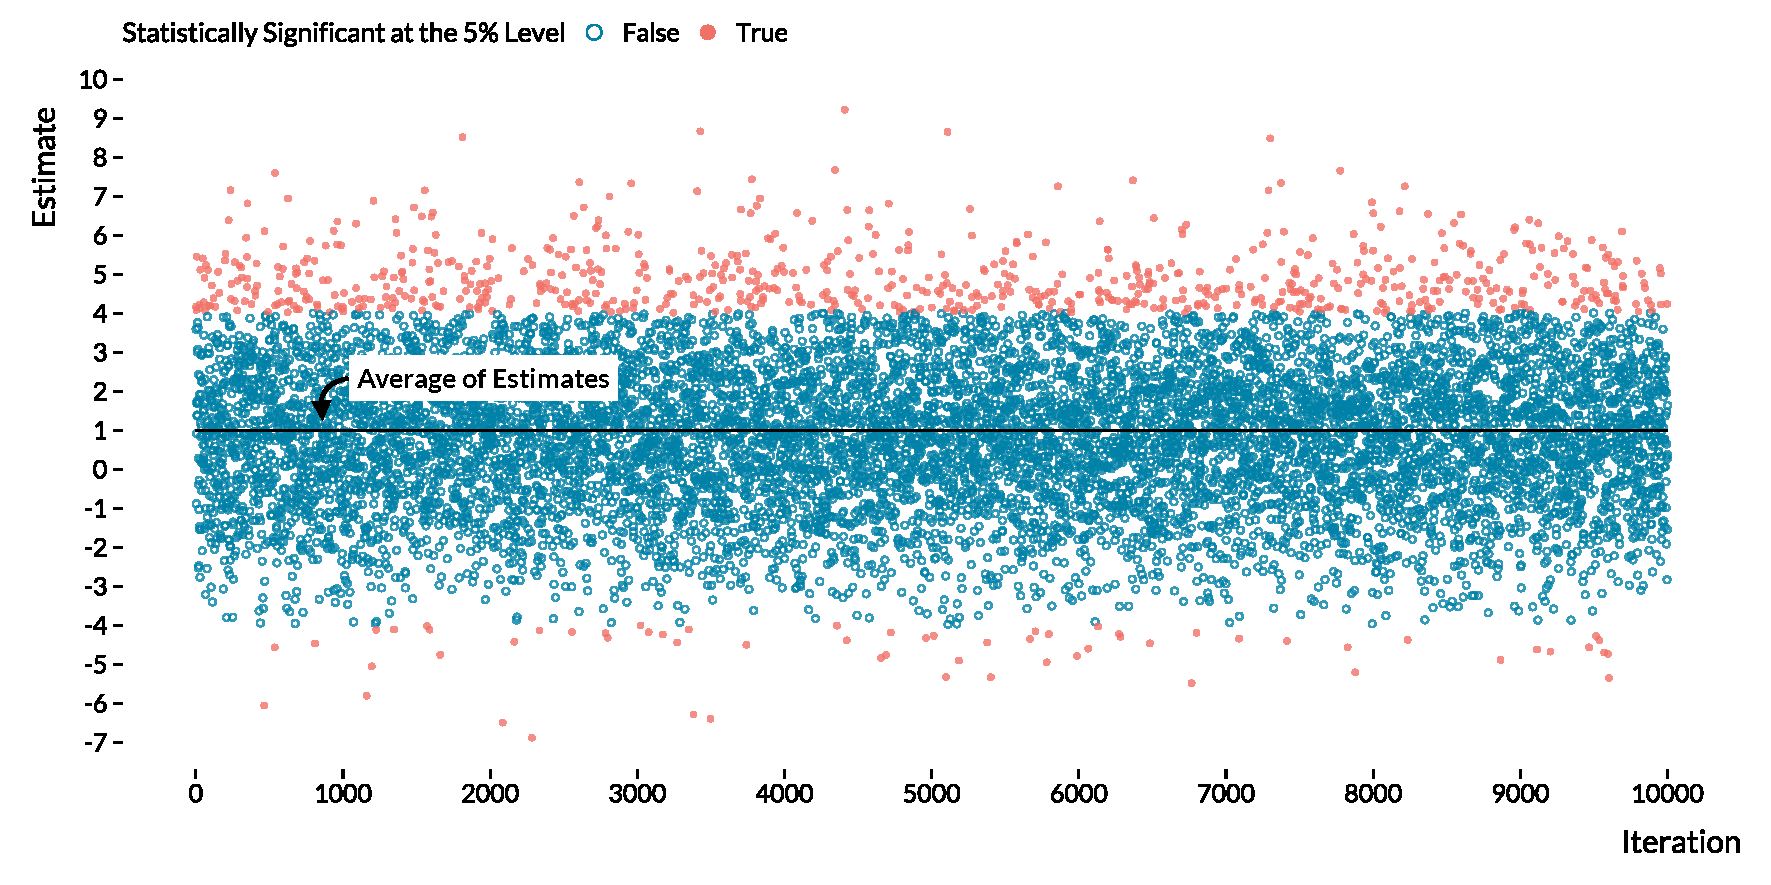
\includegraphics[width=\linewidth]{images/graph_experiment_results.pdf}
            \caption*{\footnotesize \textnormal{\textit{Notes}: Each dot represents a point estimates of one of the 10,000 iterations of the randomized experiment ran by the mad scientist. Red dots are statistically significant at the 5\% level while blue dots are not. The black solid line represents the average of estimates, equal to the true average effect of 1 additional death.}}
        \end{figure}
    
    With such a low statistical power, statistically significant estimates are however not informative of the treatment of interest. Two metrics, the average type M (magnitude) error and the probability to make a type S (sign) error help assess the negative consequences of a lack of statistical power. The exaggeration ratio, or expected type M error, is defined as the ratio of the absolute values of the statistically significant estimates over the true effect size \citep{gelman_beyond_2014}. In the present case, with an estimated statistical power of 8\%, the scientist could expect their statistically significant estimates to be inflated on average by a factor of 5. We also notice in \Cref{fig:estimates_experiments} that a non-negligible fraction of statistically significant estimates are of the wrong sign: this proportion is the probability of making a type S error \citep{gelman_type_2000}. In this experiment, a statistically significant estimate has a 8\% probability of being of the wrong sign. 
    
    Formally, the statistical power of a test is the probability of rejecting the null hypothesis $H_{0}: \beta = 0$, where $\beta$ is the true effect of the estimand of interest. For $\hat{\beta}$, a normally distributed unbiased estimate of $\beta$ with standard error $\sigma$, the power of the null hypothesis test at the 5\% level is equal to $\Phi\left(-1.96-\frac{\beta}{\sigma}\right)+1-\Phi\left(1.96-\frac{\beta}{\sigma}\right)$, where $\Phi$ is the cumulative distribution function of the standard normal distribution. It increases with $\beta$, the true value of the effect and with the precision of the estimate, \textit{i.e.}, when $\sigma$ decreases. The exaggeration ratio is $\mathbb{E}\left(\frac{|\hat{\beta}|}{|\beta|} \ \bigg| \ \beta, \sigma, |\hat{\beta}|/\sigma>1.96\right)$ and the probability to make a type S error is given by $\text{Pr}\left(\frac{\hat{\beta}}{\beta} < 0 \ \bigg| \ \beta, \sigma, |\hat{\beta}|/\sigma>1.96 \right)$.  \cite{zwet_significance_2021} and \cite{lu_note_2019} derive closed-form expressions for these quantities. They show that both the exaggeration ratio and the probability of type S error decrease with $\beta$ and the precision of the estimate and thus with statistical power. %, and thus increase with $\sigma$. 
    %. In addition, they show that the lower the statistical power, the larger the exaggeration and the probability of type S error.

    To obtain statistically significant estimates that are informative of the true value of the effect size, the scientist would need to improve the design of their study in order to increase its statistical power. %Also note that a low statistical power does not allow pinpointing erroneous estimates as such. This can lead to inflated reported estimates even in the absence of a significance filter, for instance when large results are favored or when there are incentives to produce estimates that differ from previous findings.  
    
	\subsection{Exaggeration of Published Estimates in Economics}
	
		The exaggeration of significant estimates matters only when certain types of results, such as statistically significant ones, are favored for publication. When statistical power is low, significant estimates constitute a non-representative subset of the estimates compatible with the data. If a publication bias favors these estimates, published estimates will exaggerate true effect sizes. Now, such selection on significance is well documented in economics \citep{rosenthal_file_1979, brodeur_star_2016, andrews_identification_2019, vivalt_specification_2019, abadie_statistical_2020, brodeur_methods_2020}, making inflated significant estimates a key issue for the discipline. Importantly, publication bias may also extend beyond significance: large or surprising results may be favored, further amplifying exaggeration when power is limited. The combination of low statistical power and publication bias appears to generate substantial and widespread exaggeration in the discipline; \citet{ioannidis_power_2017} estimate that nearly 80\% of results across a wide array of economics literatures are exaggerated by a factor of two or more. In the following sections, we explore exaggeration and power issues in the literature of interest, complementing prior assessments of exaggeration in economics through a focus on causal identification approaches. This quantification enables us to document the potential impacts of exaggeration on the design of public policies.
			
%------------------------------------------------------------------------------

% RETROSPECTIVE DESIGN ANALYSIS OF THE LITERATURE

%------------------------------------------------------------------------------

\section{Quantifying Exaggeration}\label{section_lit_review}

	From extreme events such as the London Fog of 1952 to the development of sophisticated time-series analyses, a vast epidemiology literature of more than 600 studies has established that air pollution induces adverse health effects over the short term. Increases in the concentration of several ambient air pollutants have been found to be associated with increases in daily mortality and emergency admissions for respiratory and cardiovascular causes \citep{schwartz_what_1994, samet_national_2000, letertre_shortterm_2002, bell_time-series_2004, liu_ambient_2019}. With this objective in mind, researchers in economics and epidemiology have recently used causal inference methods to improve on the standard epidemiology literature that relied on associations \citep{dominici_best_2017, bind_causal_2019}. Newly obtained results confirm the short-term health effects of air pollution \citep{schwartz_estimating_2015, schwartz_national_2018, deryugina_mortality_2019}. Based on these results, environmental protection and public health agencies have designed policies such as air quality alerts to mitigate the burden of air pollution. Accurate estimates of these effects are therefore crucial as they are directly used to implement and update policies to address this major public health issue.
	
	This section reviews this literature through the prism of statistical power and exaggeration, with particular focus on causal approaches. It describes how we ran retrospective analyses of the causal inference and standard epidemiology literatures as well as steps we undertook to make this analysis easily reproducible in other literatures.
    
    \subsection{Approach}
    
        The formulas for power, exaggeration ratio and type S error described in the previous section all depend on the true magnitude of the estimand of interest. The true effect is however never observed in a given study.  We can overcome this limitation with a retrospective power analysis. Essentially, it addresses the following question: would the design of our study be reliable enough to retrieve the true effect if it was in fact smaller than the obtained estimate? A retrospective power analysis can be considered as a thought-experiment in which we would exactly replicate the study many times under the assumption that the true effect is different from the observed estimate. The reasoning is analogous to the analysis in the previous section. Concretely, \cite{gelman_beyond_2014} propose to run simulations in which we draw many estimates from the asymptotic distribution of the estimator, a normal distribution with mean equal to the hypothesized true effect and a standard deviation equal to the standard error we obtained in the study. The statistical power is the proportion of sampled estimates that are statistically significant at the 5\% level. The exaggeration ratio is computed as the average ratio of the absolute values of statistically significant estimates over the assumed true effect size. The probability to make a type S error is the proportion of significant estimates that are of the opposite sign of the true value. In this project, we use the \textbf{\textsf{R}} package \texttt{retrodesign} described in \cite{timm_retrodesign_2019} that implements the closed-form analogue of these simulations \citep{lu_note_2019}.
    
        To get a general overview of power issues in the causal inference and standard epidemiology literatures, we first carry out a simple retrospective analysis for each study. These computations rely on hypothesized true effect sizes. Yet, since treatments and outcomes vary between studies in this literature, it is not possible to make general aggregated assumptions on true effect sizes. We need to consider specific hypothesized true effect sizes for each study. Since \cite{ioannidis_power_2017} and \cite{ferraro_feature_2020} find a typical exaggeration of two in the economics literature, we evaluate the proportion of studies that would have a design reliable enough to retrieve an effect size equal to half of the obtained estimate. We do not claim that the hypothesized effect size is the true effect size but rather wonder whether the design of the study would allow capturing an effect of this magnitude. A well-designed study should be able to detect a range of plausible effect sizes that are smaller than the observed estimate. This method is however by no means ideal but offers some sort of consistency across studies. To overcome this limitation, for a subset of studies, we also use results from a meta-analysis as potential values for the true effect sizes. 

    % CAUSAL INFERENCE LITERATURE
    \subsection{Exaggeration in the Causal Inference Literature}
    
        
       % search strategy and number of studies retrieved
        For the causal inference literature, an extensive search strategy on \href{https://scholar.google.com/}{Google Scholar}, \href{https://ideas.repec.org/}{IDEAS}, and \href{https://pubmed.ncbi.nlm.nih.gov/}{PubMed} enables retrieving studies that (i) focus on the short-term health effects of air pollution on mortality and morbidity outcomes, and (ii) rely on a causal inference methods\footnote{The very recent literature on the effects of air pollution on COVID-19 health outcomes is excluded to gather a relatively homogeneous corpus of studies.}. Appendix \ref{causal_lit} displays the list of the 36 articles that match the search criteria. For each study, we manually retrieve the method used by the authors, the health outcome and air pollutant they consider, the point estimate and the standard error of the main specifications.%We also consider the results on heterogeneous effects by age categories. 
        
        To evaluate potential statistical power issues in this literature, we follow the same approach as for the analysis of the standard epidemiology literature. \Cref{fig:retro_causal} plots the power and exaggeration curves for 186 specifications which results are statistically significant at the 5\% level. If the true effect size of each study was equal to half of the obtained estimate, the median power would be 33\% and the median exaggeration ratio would be 1.7. Only 11\% of studies would have a power greater than 80\%. \Cref{fig:retro_causal} also shows that there is a wide heterogeneity in statistical power issues among studies. Some of them are estimated to be relatively well powered while others can run into large exaggeration issues. For instance, one quarter of studies would, on average, exaggerate the true effect sizes by a factor greater than 2. This pattern may help explain the very large effect sizes sometimes observed in the causal inference literature. 

          \begin{figure}[ht!]
            \caption{Statistical Power and Exaggeration Curves of Causal Inference Studies.}
            \label{fig:retro_causal}
        \centering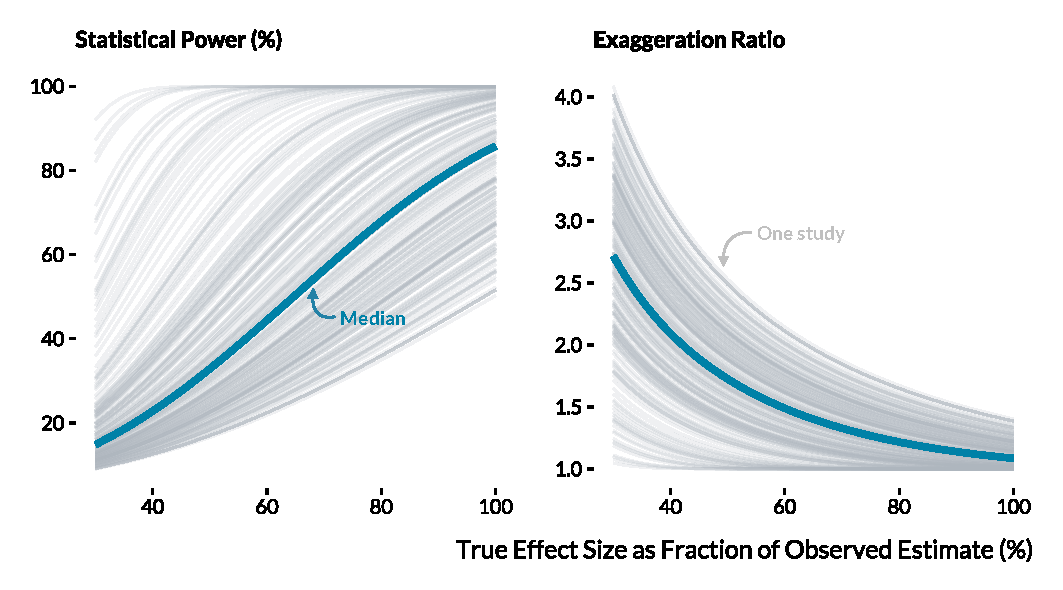
\includegraphics[width=\linewidth]{images/graph_retrodesign_causal_inf.pdf}
            \caption*{\footnotesize \textnormal{\textit{Notes}: Each gray line is a power curve or an exaggeration curve of a statistically significant result published in the causal inference literature. The blue lines are the median values. For visual clarity, we drop results for which exaggeration ratios were too large.}}
        \end{figure}
        
        %As for the epidemiology literature, we can get an overview of power issues in the causal inference literature by considering the ability of studies to detect effects sizes equal to half of observed estimates. However this choice remains arbitrary. To make more informed guesses about the values of true effect sizes, we use the estimates that epidemiologist would have predicted using non-causal inference methods. We focus on instrumental variable strategies since they are the most common design in the causal inference literature. The discrepancy between OLS and 2SLS estimates is often explained by a combination of omitted variable bias and attenuation bias due to classical measurement error in air pollution exposure. It can also come from the fact that the causal estimands targeted by both strategies are different when treatment effects are heterogeneous. There is however a lack of evidence on the contribution of each explanation to the discrepancy between non-causal and causal estimates. 
        
        Then, for the 49 instrumental variable results that are statistically significant and reporting the corresponding naive regression results, we can evaluate whether the 2SLS specifications would recover a true effect closer to that of the naive estimate. \Cref{fig:retro_iv} displays the distribution of the resulting statistical power and the average exaggeration ratio. The median estimated power is equal to 8.4\%. This results in very large exaggeration ratios: half of the studies would exaggerate a true effect of the size of the OLS estimate by a factor of at least 4.5. Some designs are also associated with extremely large exaggeration ratios, larger than 8.2 for a quarter of them. Such an inflation of statistically significant estimates could explain part of the gap between the standard and causal literature. This discrepancy could also be explained by a combination of omitted variable bias and attenuation bias caused by classical measurement error in air pollution exposure. It could also come from the fact that the causal estimands targeted by both strategies are different when treatment effects are heterogeneous. Such explanations are not mutually exclusive and the lack of power and inability of the instrumental variables to recover smaller effect sizes remain concerning. In the presence of publication bias, considerable lack of power mechanically causes substantial exaggeration issues.
        
        \begin{figure}[ht!]
            \caption{Distribution of Power and Exaggeration Ratio for Instrument Variable Designs, Assuming that the Naive OLS Estimates Are the True Effect Sizes.}
            \label{fig:retro_iv}
        \centering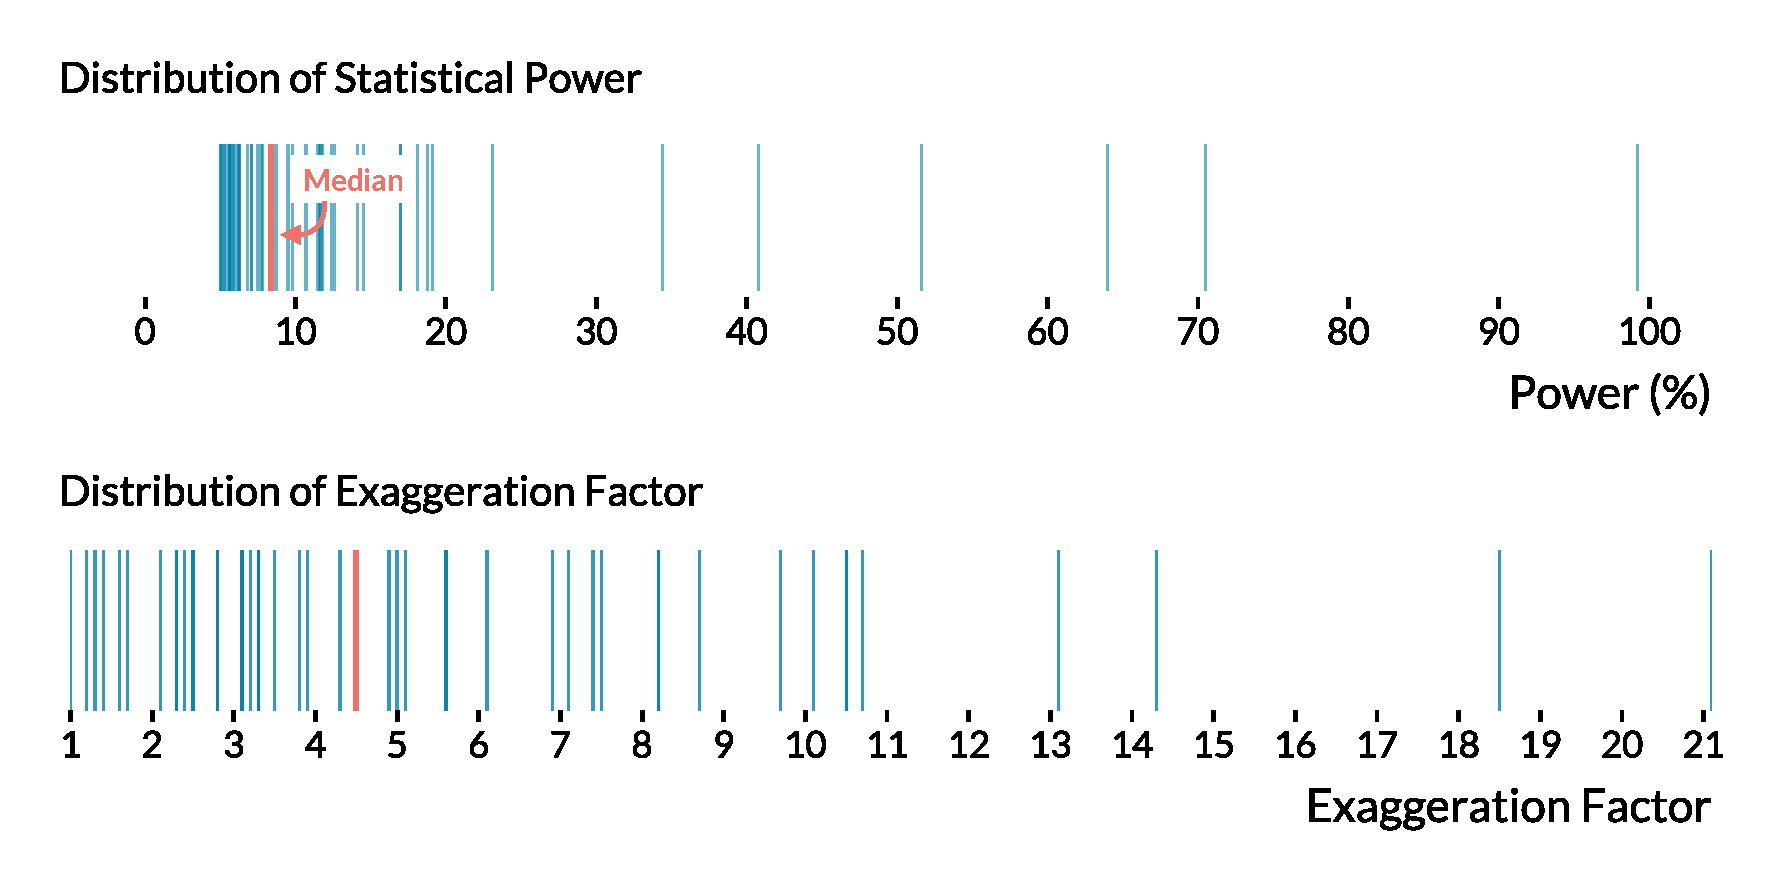
\includegraphics[width=\linewidth]{images/graph_retro_iv.pdf}
            \caption*{\footnotesize \textnormal{\textit{Notes}: For 49 statistically significant 2SLS estimates, we define the true values of effect size as the corresponding OLS estimates. Each blue line represents either the estimated statistical power (\%) or exaggeration factor of a study's result. Orange lines are the median of the two metrics. For visual clarity, we do not display three extreme exaggeration ratios.}}
        \end{figure}
                
        Exaggeration arises when significant results are favored. The left panel of \Cref{fig:intro} reveals its presence for the causal literature. As in \cite{brodeur_star_2016, brodeur_methods_2020} for the broader economics literature, there is an excess mass in the \textit{t}-statistics distribution at the 5\% statistical significance threshold. The right panel of \Cref{fig:intro} produces further evidence of this favoring of significant estimates but also  points to a consequence of this publication bias: published estimates from imprecise studies might be exaggerated. Imprecise designs yield larger standardized effect sizes. If published estimates captured true effects, their standardized effect size should be independent of the precision of the study. This figure constitutes suggestive evidence of both selection on significance and exaggeration in this literature.

        \begin{figure}[ht!]
            \caption{Suggestive Evidence of Publication Bias and Exaggeration in the Causal Inference Literature on Acute Health Effects of Air Pollution.}
            \label{fig:intro}
            \centering
            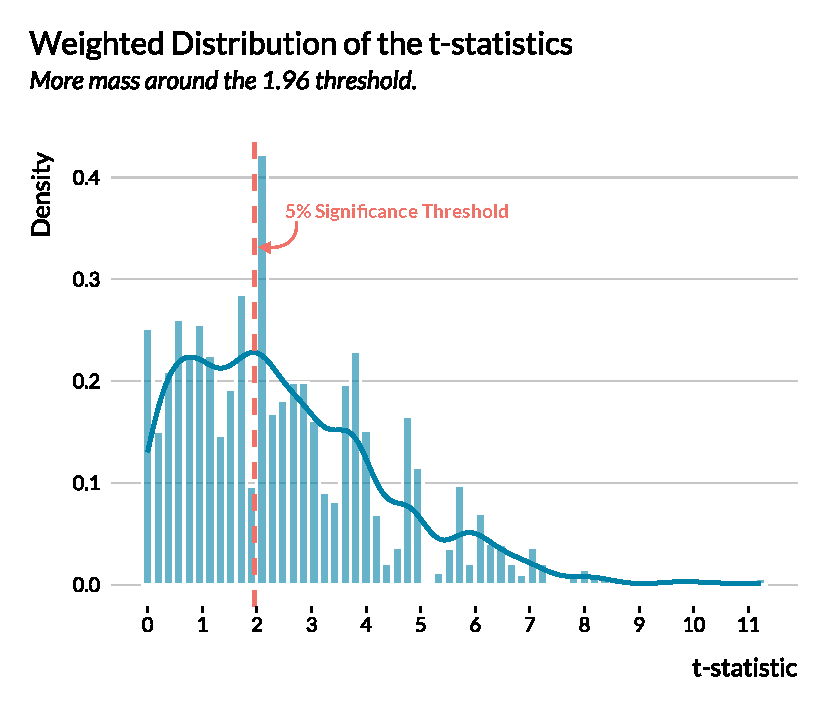
\includegraphics[width=0.48\linewidth]{images/graph_distribution_t.pdf} \ 
            \includegraphics[width=0.48\linewidth]{images/graph_effect_precision.pdf}
            \caption*{\footnotesize \textnormal{\textit{Notes}: The sample in the left panel includes all 537 estimates reported in articles from the causal literature, including ``naive'' OLS estimates and placebo tests. Following \cite{brodeur_methods_2020}, the weights are equal to the inverse of the number of tests displayed in the same table multiplied by the inverse of the number of tables in the article. In the right panel we exclude the ``naive''  OLS estimates and placebo tests. Both axes are on a log10 scale. Limiting the sample to economics journal leaves the figures essentially unchanged (see  supplemental material). Distinguishing between top 5 and other journals shows that even if there  standardized effect sizes are typically smaller in top 5 journals, the same inverse relationship can be observed.}}
        \end{figure}
    
    % EPIDEMIOLOGY LITERATURE
    \subsection{Exaggeration in the Standard Epidemiology Literature}
    
        % introductory paragraph
        Hundreds of papers have been published on the short-term health effects of air pollution in epidemiology, medicine and public health journals. A large fraction of articles rely on Poisson generalized additive models, which allow flexibly adjusting for the temporal trend of health outcomes and for non-linear effects of weather parameters. This literature spans over 20 years and has replicated analyses in a large number of settings, providing crucial insights on the acute health effect of air pollution. 
    
        To gather a corpus of relevant articles, we use the following search query on \href{https://www.ncbi.nlm.nih.gov/}{PubMed} and \href{https://www.scopus.com/home.uri}{Scopus}:
               
        \begin{quote}
       \footnotesize\texttt{'TITLE(("air pollution" OR "air quality" OR "particulate matter" OR "ozone"', 'OR "nitrogen dioxide" OR "sulfur dioxide" OR "PM10" OR "PM2.5" OR', ' "carbon dioxide" OR "carbon monoxide")',  'AND ("emergency" OR "mortality" OR "stroke" OR "cerebrovascular" OR', '"cardiovascular" OR "death" OR "hospitalization")', 'AND NOT ("long term" OR "long-term")) AND "short term"'}
        \end{quote}

       \noindent We retrieve the abstracts of 1834 articles. Then, we extract estimates and confidence intervals from these abstracts using regular expressions (regex). Our algorithm available \href{https://vincentbagilet.github.io/inference_pollution/automatic_lit_review_getting_abstracts.html}{online} detects phrases such as “95\% confidence interval (CI)” or “95\% CI” and looks for numbers directly before this phrase or after and in a confidence interval-like format. We illustrate the outcome of this procedure (in blue) using one sentence of a randomly selected article from this literature review \citep{vichit-vadakan_public_2008}:
        
\begin{sloppypar}
        \begin{quote}
         \footnotesize    “\texttt{The excess risk for non-accidental mortality was \textbf{\color{cerulean}1.3\% [95\% confidence interval (CI), 0.8–1.7]} per 10 $\mu \text{g/m}^3$ of PM10, with higher excess risks for cardiovascular and above age 65 mortality of \textbf{\color{cerulean}1.9\% (95\% CI, 0.8–3.0)} and \textbf{\color{cerulean}1.5\% (95\% CI, 0.9–2.1)}, respectively.}”
        \end{quote}
\end{sloppypar}

        \noindent Using this reproducible method, we retrieve 2666 estimates from 784 abstracts. We then read these abstracts and filter out articles whose topic falls outside of the scope of our literature review. The final corpus is thus composed of 668 articles and 2155 estimates. Importantly, the set of articles considered is limited to those displaying confidence intervals and point estimates in their abstracts. We also build regex queries to retrieve other information about the articles such as the air pollutant and health outcome studied, the length of the study and the number of cities considered.
            
        Based on this subset of articles, we first implement a retrospective power analysis to evaluate whether a study could recover an effect size equal to half of the obtained estimate. We carry out this analysis for the 1982 estimates that are statistically significant. \Cref{fig:retro_epi} displays the power and exaggeration curves for each result. They describe how these metrics vary with the hypothetical true effect sizes. 

         \begin{figure}[ht!]
                \caption{Power and Exaggeration Curves for the Epidemiology Literature.}
                \label{fig:retro_epi}
                \centering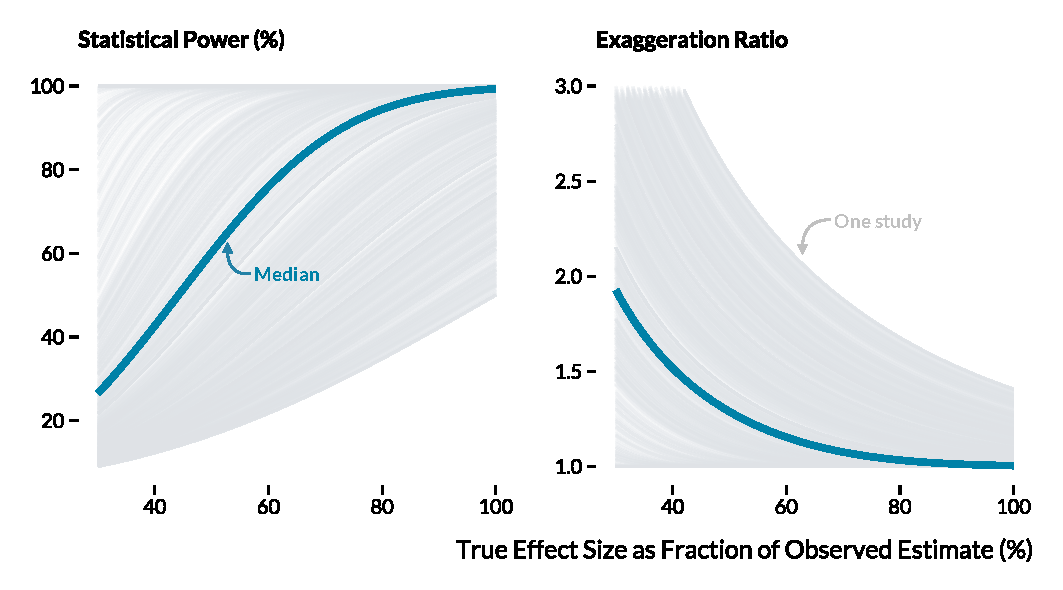
\includegraphics[width=\linewidth]{images/graph_retrodesign_epi.pdf}
                \caption*{\footnotesize \textnormal{\textit{Notes}: Each gray line is a power curve or an exaggeration curve of a statistically significant result published in the epidemiology literature. The blue lines are the median values. For visual clarity, we drop results for which exaggeration ratios were too large.}}
            \end{figure}
        
        If the true effect size was equal to half of the obtained estimate, 58\% of the studies would have a power below the conventional 80\% target used in randomized controlled trials. The median exaggeration ratio would be 1.3 and type S error would not be an issue. These figures however hide a lot of heterogeneity across studies. For one quarter of studies, the exaggeration would be higher than 1.9. We therefore try to apprehend the sources of this heterogeneity.
    
        We find that inference issues do not depend on the health outcome and the air pollutant studied. Health science journals appear to be less prone to power issues than other journals. Researchers seem to be aware that they should work with large sample size as they often carry out multi-city studies. They also sometimes explicitly state that they investigate non-accidental mortality causes to increase statistical power since the average daily count is higher than for more specific death causes. Yet, the proportion of low power studies has been stagnating since the 2000s, revealing that practices regarding statistical power have not evolved. 

        Studying the ability of each study to detect an effect that would be half of the obtained estimate gives an overview of power issues in this literature. It can however be viewed as arbitrary. Besides, while our approach enables studying the whole literature, it does not allow clearly analyzing the type of pollutants and outcomes considered in each study. As recommended by \cite{gelman_beyond_2014} and \cite{ioannidis_power_2017}, we thus make more informed guesses about potential true effect sizes for a subset of the literature using results from a meta-analysis. \cite{shah_short_2015} gathered 94 studies on the effects of several air pollutants on mortality and emergency admission for stroke. For each of these studies, we run retrospective power calculations to evaluate their ability to retrieve the meta-analysis estimates. We find that 63\% of the studies in \cite{shah_short_2015} have an estimated statistical power below 80\%. The median estimated exaggeration ratio of statistically significant estimate is equal to 1.6. \Cref{fig:retro_meta_epi} plots for each air pollutant, the distribution of the exaggeration ratios (blue lines) and their medians (orange lines). The median estimated exaggeration varies a lot by air pollutant, from 1 for PM$_{2.5}$ up to 13.4 for O$_{3}$ (the median is not displayed for visual clarity). More informed guesses about true effect sizes confirm that exaggeration is common in the standard epidemiology literature.

        \begin{figure}[ht!]
            \caption{Distribution of Exaggeration Ratios for Studies in \cite{shah_short_2015}'s Meta-Analysis.}
            \label{fig:retro_meta_epi}
            \centering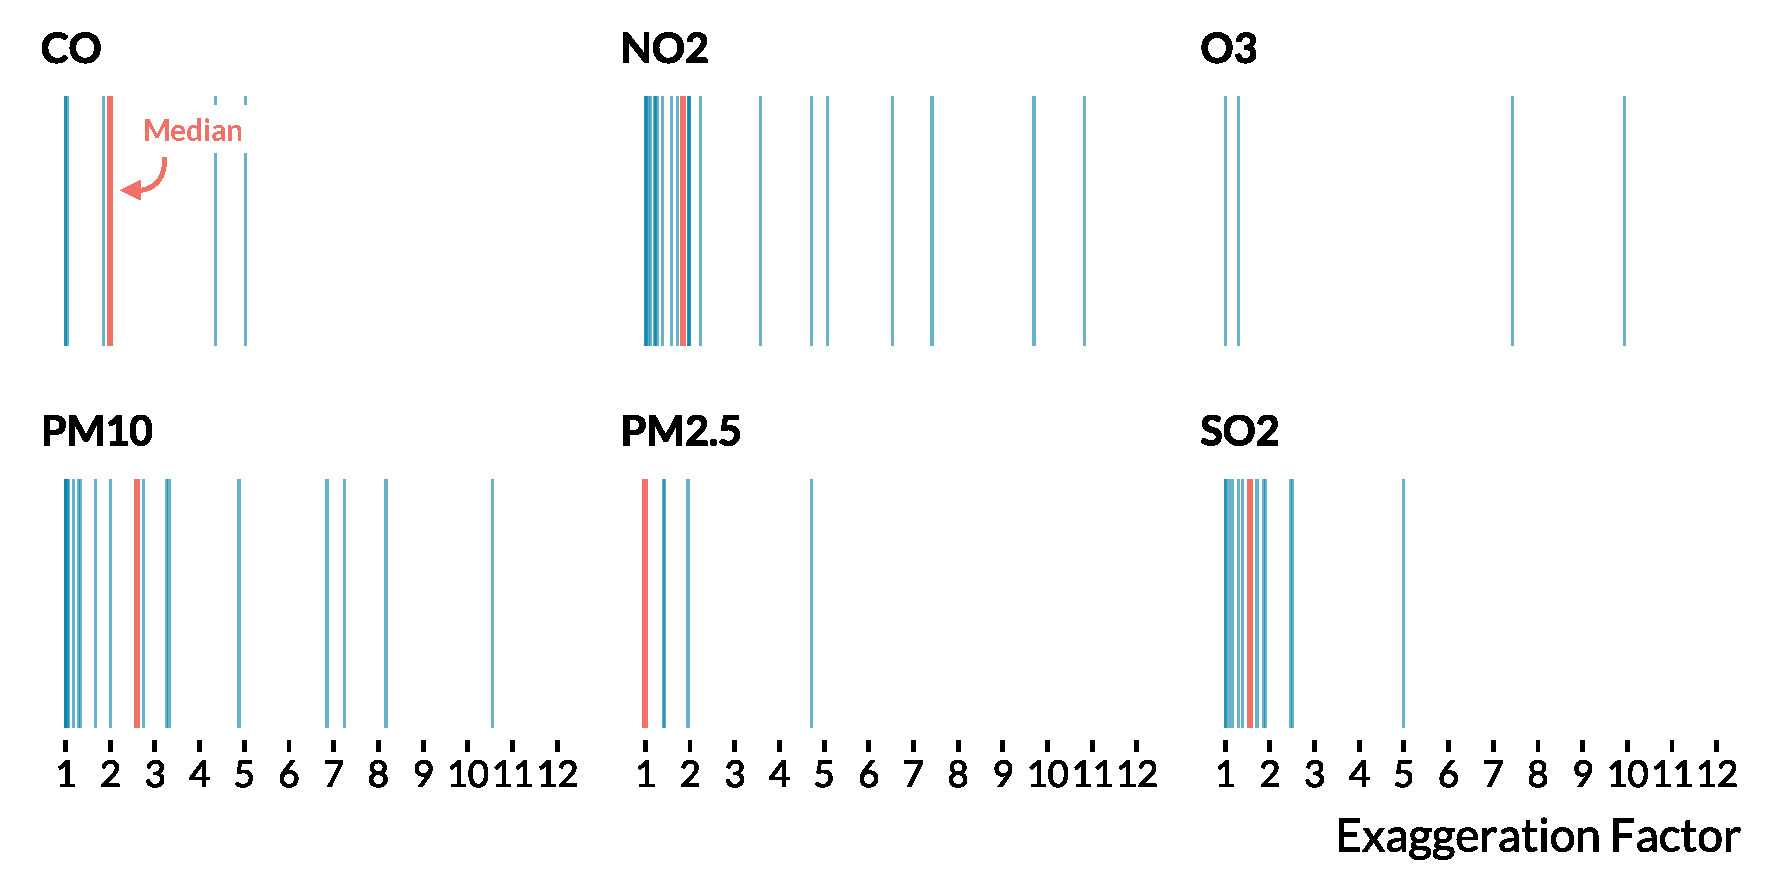
\includegraphics[width=0.9\linewidth]{images/graph_shah_2015.pdf}
            \caption*{\footnotesize \textnormal{\textit{Notes}: Each blue line is the exaggeration ratio of a statistically significant estimate retrieved from \cite{shah_short_2015}'s meta-analysis. We use the meta-analysis estimates as true effect sizes in the retrospective power calculations. Orange lines are the medians. Extreme exaggeration ratios are removed for visual clarity. The median for O$_{3}$ is 13.4.}}
        \end{figure}

        In this corpus and contrarily to the causal inference corpus, we do not observe the entire universe of published estimates but a selected subset: those that are reported in the abstracts. We can however evaluate a particular form of selection on significance, through the selection of headline results. These estimates are the ones that are emphasized and that thus may be used to inform policymaking. As visible on \Cref{fig:distrib_t_stat_epi}, there is a striking bunching at the 1.96 threshold. Statistically significant results are favored in this literature, at least in terms of selection of results put forward. Identification approaches being rather uniform in this literature, the results may be particularly central in the assessment of the quality of a study and may play a central role in the decision process for publication. 

        \begin{figure}[ht!]
            \caption{Distribution of t-statistics of estimates in abstracts from the standard epidemiology literature}
            \label{fig:distrib_t_stat_epi}
            \centering\includegraphics[width=0.8\linewidth]{images/distrib_t_stat_epi.pdf}
            \caption*{\footnotesize \textnormal{\textit{Notes}: All estimates come from the abstracts. Estimates with t-stat > 10 are not reported here for readability. The vertical dashed line represents the usual 1.96 threshold.}}
        \end{figure}
        
%------------------------------------------------------------------------------

% Impacts of Exaggeration on Public Policy

%------------------------------------------------------------------------------

\vspace{-0.5cm}
\section{Impacts of Exaggeration on Public Policy}\label{section_policy}

	The estimates produced by academic studies frequently inform regulatory decisions. This section explores the impacts of exaggeration on the design of concrete public policies through the example of air pollution mitigation policies in the United States, drawing on the results from the exploration of the literature from the previous section. While the policy analysis focuses on a specific topic, the intuitions extend to other settings where academic estimates inform policy. 

	\subsection{Academic Estimates Enter the Design of Public Policy}

		Under the Clean Air Act, the EPA sets National Ambient Air Quality Standards (NAAQS) based on systematic reviews of the scientific literature, synthesized in Integrated Science Assessments (ISAs) \citep{u.s.epa_preamble_2015}.\footnote{This reflects the regulatory framework in place through the end of 2024; more recent executive actions have lessened the emphasis on quantifying health impacts in some regulatory decision contexts.} Beyond standard-setting, academic estimates enter the cost-benefit analyses of major regulations through Regulatory Impact Analyses (RIAs), which compare the social costs and monetized benefits of alternative regulatory approaches \citep{u.s.epa_final_2024}. To quantify health benefits, the EPA relies on the Benefits Mapping and Analysis Program (BenMAP-CE), a modeling tool that combines air quality projections with concentration-response coefficients drawn from the epidemiology literature to estimate the economic value of changes in air pollution concentrations \citep{sacks_environmental_2018}. States are responsible for implementing these standards through State Implementation Plans (SIPs), and often draw on EPA-provided analytical tools such as BenMAP-CE, as well as guidance from RIAs and associated technical documents, to select compliance measures \citep{u.s.epa_environmental_2023}.
		
		In BenMAP-CE, health benefits from air quality improvements are computed in several steps \citep{sacks_environmental_2018}. After modeling changes in air pollution, the software relates them to changes in health outcomes using concentration-response functions derived from the epidemiological literature. These studies typically estimate log-linear concentration-response functions: $\Delta Y = \text{Pop} \times Y_0 \times (1 - e^{-\hat{\beta} \times \Delta AQ})$ where $\Delta Y$ denotes the change in health outcomes attributed to air pollution, Pop the exposed population, $Y_0$ the baseline incidence, $\Delta AQ$ the specified change in air quality, and $\hat{\beta}$ the estimated health effect coefficient. For the small concentration changes typically considered in regulatory analysis, this simplifies to $\Delta Y \approx \text{Pop} \times Y_0 \times \hat{\beta} \times \Delta AQ$. The economic value of avoided health effects is then computed by multiplying $\Delta Y$ by an estimate of the economic value of this health effect, \textit{e.g.}, for mortality, the Value of a Statistical Life (VSL), whose central estimate recommended by the EPA is approximately \$10.7 million in 2022 dollars.\footnote{EPA's central VSL estimate of \$4.8 million (1990\$) adjusts to approximately \$10.7 million with the Consumer Price Index \citep{u.s.epa_guidelines_2024}.} These monetized benefits can then be compared against abatement costs to compute the net benefits of alternative policies. 


	\subsection{Policy Implications of Exaggeration}
		
		We now assess the policy implications of exaggeration. In the specification of health effects mentioned above, monetized health benefits are proportional to the true health effects $\beta$. If the estimated health effects are exaggerated by a factor $\zeta = \frac{\hat{\beta}}{\beta}$, perceived benefits will be exaggerated by the same factor. To explore concrete implications on policy, consider the 2024 RIA for the revision of the PM$_{2.5}$ standards, which lowered the annual standard from 12 to 9 $\mu\text{g/m}^3$ \citep{u.s.epa_final_2024}. The RIA estimates annual monetized benefits in 2032 between \$22 billion and \$46 billion (2017\$) against annual costs of \$590 million.  %eg cf table ES-10
		These health benefits are explicitly derived from a review of academic studies and calculated using BenMAP-CE.  %eg cf table ES-6
		Given that the benefits of regulation outweigh costs by more than an order of magnitude, even substantial exaggeration leading to inflated perceived benefits would not eliminate positive net benefits. However, true net benefits would be lower than the regulator expects. \Cref{tab:policy_implications} describes the impact of the exaggeration ratios estimated in \Cref{section_lit_review} on the RIA benefit-costs analysis for the high expected benefit estimate of \$46 billion.
		
		\begin{table}[!ht]
	\caption{Policy Implications of Documented Exaggeration.}
	\label{tab:policy_implications}
	\centering
		\begin{threeparttable}
                		\begin{tabular}{lccccc}
                    		\toprule
                    			 & Exaggeration & Expected & Actual & Difference \\ 
			 		 & ratio & Net Benefits & Net Benefits & (B\$/year) \\ 
			 		 &  &  (B\$/year) & (B\$/year) & \\ 
				\midrule
				Epidemiology median & 1.3 & 45.4 & 34.9 & 10.5 \\
				Epidemiology 25th pctile & 1.9 & 45.4 &  23.9 & 21.5 \\
				Causal inference median & 1.7 & 45.4 & 26.7 & 18.7  \\
				Causal inference 25th pctile & 2.0 & 45.4 & 22.7 & 22.7 \\
				IV vs.\ OLS median & 4.5 & 45.4 & 10.1 & 35.3 \\
                    		\bottomrule
                \end{tabular}
                \begin{tablenotes}
                    \footnotesize
                    \item \textit{Notes}: Actual net benefits represent the net benefits under the hypothesis of exaggerated health effects: due to the linearity of the relationship between health effects and monetized benefits, they are simply computed as the expected net benefits of \$46 billion (the high estimate for the 9 $\mu\text{g/m}^3$ standard) divided by the exaggeration ratio found in our analysis of the literature. The last column represents the difference between the expected and actual net benefits.
                \end{tablenotes}
            \end{threeparttable}
\end{table}
		
		These discrepancies are economically large: annual misperceptions of net benefits range from \$10.5 to \$35.3 billion. Policy makers relying on exaggerated estimates would overstate the social surplus and the economic justification for stringent standards. When benefit-cost analyses are used to compare potential regulations, systematic exaggeration of health benefits could make air quality interventions appear more attractive than alternative health policies that may yield higher returns. The same logic applies when comparing different standard levels. If exaggeration varies across standards, for instance due to differences in the exposure ranges, the ranking of options may be affected even when all generate positive net benefits.
		
		The acute health effects literature provides an ideal setting for studying the drivers of exaggeration but is less well suited for illustrating its policy consequences. Air pollution regulations have benefit-cost ratios around 50, large enough that even substantial exaggeration leaves net benefits positive. In domains where estimated benefits and costs are closer in magnitude, the exaggeration ratios documented in \Cref{section_lit_review} could plausibly flip the sign of a benefit-cost analysis and therefore affect whether a regulation is implemented.
		
				
%	\subsection{A Simple Welfare Analysis}
%	
%		To quantify the welfare consequences of exaggeration, consider a textbook model of pollution abatement. A regulator chooses an abatement level $a$ to maximize net benefits, where benefits are $B(a) = b a$ and abatement costs are $C(a) = \frac{1}{2}c a^2$.\footnote{The assumption of linear benefits is consistent with the aforementioned modeling. The assumption of convex abatement costs is standard and consistent with observed marginal abatement cost curves, though actual abatement cost curves used by the EPA in RIAs are step functions reflecting discrete control technologies rather than smooth quadratics.} The parameter $b$ combines VSL, population, baseline mortality, and the true health effect $\beta$. If the regulator knew the true marginal benefit $b$, they would equate it to marginal costs, setting an abatement level $a^{\textsc{fb}} = b/c$. This yiels first-best welfare $W^{\textsc{fb}} = B(a^{\textsc{fb}}) - C(a^{\textsc{fb}}) = \frac{b^{2}}{2c}$. However, if the health effect estimate is exaggerated, perceived benefits are $\hat{B}(a) = \hat{b} a = \zeta b a$ and the regulator chooses $a^{*} = \zeta b/c = \zeta a^{\textsc{fb}}$, over-abating relative to the first-best by a factor equal to the exaggeration ratio. This yields welfare $W^{*} = B(a^{*}) - C(a^{*}) = \frac{b^{2}}{2c}(2\zeta - \zeta^2)$ and thus a welfare loss of:
%		
%		\begin{equation} 
%			L(\zeta) = W^{\textsc{fb}} - W^{*} = W^{\textsc{fb}}(\zeta - 1)^2
%		\end{equation}
%		
%		This quadratic structure has major implications: in this stylized framework, an exaggeration ratio of 2 implies complete elimination of net welfare gains from regulation. Nevertheless, in a more realistic setting the consequences of 
		
%------------------------------------------------------------------------------

% SECTION - PROSPECTIVE ANALYSIS OF CAUSAL INFERENCE STRATEGIES 

%------------------------------------------------------------------------------

\section{Approach for the Prospective Analysis}\label{section_simulations}

    While a literature review can provide evidence of exaggeration and lack of statistical power, it does not allow us to clearly identify the parameters driving it. We therefore implement a prospective analysis to overcome this limitation \citep[for other examples of power simulations]{altoe_enhancing_2020, black_simulated_2022}. We run Monte-Carlo simulations based on real-data to emulate the main empirical strategies found in the literature. We use real data to avoid the difficult task of modeling the long-term and seasonal variations in health outcomes but also the specific effects of weather variables such as temperature. These simulations are grounded in the literature on the acute health effects of air pollution but share nonetheless many similarities with prevailing applied economics settings; panel data, large data sets, canonical identification strategies.
    
    The present section describes how the simulations are implemented. Before that, we present the causal identification strategies used to measure the acute health effects of air pollution and then briefly describe the data used for the simulations.
        
    \subsection{Research Designs to Measure the Short-Term Health Effects of Air Pollution}
        
        Several empirical strategies have been leveraged to estimate the short-term health effects of air pollution. We simulate the main ones existing in the literature. We consider the usual setting where data on air pollution, weather parameters, and health outcomes are at the daily-city level.
        
        \begin{sloppypar}
        \paragraph{Standard regression approach.} The standard strategy consists in directly estimating the dose-response between an air pollutant and an health outcome. In the epidemiology literature, researchers often rely on Poisson generalize additive models where they regress the daily count of an health outcome on an air pollutant concentration, while flexibly adjusting for weather parameters, seasonal and long-term variations. We approximate the workhorse model used by epidemiologists using linear models estimated via ordinary least squares:
        ~
        \begin{equation}
            \text{Y}_{c,t} = \alpha + \beta\text{P}_{c,t} + \textbf{W}_{c,t}\lambda + \textbf{C}_{t}\gamma + \epsilon_{c,t}
        \end{equation}
        \end{sloppypar}
        
        \noindent where $c$ is the city index and $t$ the daily time index. $\text{Y}_{c,t}$ is the daily count of cases of an health outcome and $\text{P}_{c,t}$ the average daily concentration of an air pollutant and $\epsilon_{c,t}$ an error term. The parameter $\beta$ captures the short-term effect of an increase in the air pollutant concentration on the health outcome. To address confounding issues, the model adjusts for a set of weather covariates,  $\textbf{W}_{c,t}$, and calendar indicators $\textbf{C}_{t}$. 
        
        \begin{sloppypar}
        \paragraph{Instrumental variable (IV) approach.} The standard strategy could be prone to omitted variable bias and measurement error. A growing number of articles therefore exploits exogenous variations in air pollution. Most causal inference papers rely on IV designs where the concentration of an air pollutant is instrumented by thermal inversions \citep{arceo_does_2016}, wind patterns \citep{schwartz_national_2018, deryugina_mortality_2019}, extreme natural events such as sandstorms or volcano eruptions \citep{ebenstein_particulate_2015, halliday_vog_2019}, or variations in transport traffic \citep{moretti_pollution_2011, knittel_caution_2016, schlenker_airports_2016}. This approach can be summarized with a two-stage model where the first stage is: 
        ~
        \begin{equation}
        \text{P}_{c,t} = \delta + \theta\text{Z}_{c,t} + \textbf{W}_{c,t}\eta + \textbf{C}_{t}\kappa + e_{c,t}
        \end{equation}
        \end{sloppypar}
        
        \noindent where $\text{Z}_{c,t}$ is the instrumental variable. The second stage is then:
        ~
        \begin{equation}
        \text{Y}_{c,t} = \alpha + \beta\widehat{\text{P}}_{c,t} + \textbf{W}_{c,t}\lambda + \textbf{C}_{t}\lambda + \epsilon_{c,t}
        \end{equation}
        
        \noindent where $\widehat{\text{P}}_{c,t}$ is the exogenous variation in an air pollutant predicted by the instrument. The causal effect measured by this approach is a weighted average of per-unit causal responses to an increase in the concentration of an air pollutant \citep{angrist_two-stage_1995}.

        \paragraph{Reduced-form approach.} A subset of articles directly estimates the relationship between the health outcome and exogenous shocks to air pollution. For instance, articles using this approach exploit public transport strikes or thermal inversion as exogenous shocks \citep{bauernschuster_when_2017, jans_economic_2018, godzinski2019short, giaccherini_when_2021}. They estimate a model of the form:
        ~
        \begin{equation}
        \text{Y}_{c,t} = \alpha + \beta\text{D}_{c,t} + \textbf{W}_{c,t}\lambda + \textbf{C}_{t}\gamma + \epsilon_{c,t}
        \end{equation}
        
        \noindent where $D_{c,t}$ is a dummy equal to 1 when city $c$ is affected by a shock at time $t$ and 0 otherwise. The parameter $\beta$ captures an intention-to-treat effect.

        \begin{sloppypar}
        \paragraph{Regression-discontinuity design (RDD) approach.} The last empirical strategy found in the literature measures the effects of air quality alerts with a regression-discontinuity design \citep{chen_effect_2018, anderson2022bounds}. In this approach, the following model is estimated for observations within an air pollution concentration bandwidth around the alert threshold:
        ~
        \begin{equation}
        \text{Y}_{c,t} = \alpha + \beta \textbf{1}\{P_{c,t} > P^{(a)}_{c}\} + \textbf{W}_{c,t}\lambda + \textbf{C}_{t}\gamma + \epsilon_{c,t}
        \end{equation}
        \end{sloppypar}
        
        \noindent where $P^{(a)}_{c}$ is the air pollution alert threshold for city $c$. We restrict our simulations to the case of sharp RDD. This model estimates the intention-to-treat effect of air quality alerts.  It can both capture the effect of a subsequent decrease in air pollution caused by traffic restriction policies and inhabitants' avoidance behavior. 
        
        \subsection{Data}
        
        The simulation exercises rely on a subset of the US National Morbidity, Mortality, and Air Pollution Study (NMMAPS). The dataset is publicly available and has been used in several major studies in the early 2000s to measure the short-term effects of ambient air pollutants on mortality outcomes \citep{peng2008statistical}. Specifically, we extract data at the city-day level for 68 cities over the 1987-1997 period. It corresponds to 4,018 daily observations per city, for a total sample size of 273,224 observations. We select observations on the average temperature (C°), the standardized concentration of carbon monoxide (CO), and mortality counts for several causes. We focus on CO as it is the air pollutant measured in most cities over the period and its concentration is strongly correlated to that of other pollutants such as particulate matter. Less than 5\% of carbon monoxide concentrations and average temperature readings are missing in the initial data set. We impute them using the chained random forest algorithm implemented in the \texttt{missRanger} package \citep{mayer_missranger_2019}.
        
        \subsection{Simulations Set-Up}
        
        \paragraph{General procedure.} Our simulation procedure follows 7 main steps:
        
        \begin{sloppypar}
        \begin{senumerate}
            \item Randomly draw a study period and a sample of cities.
            \item For instrumental variable, reduced-form and regression-discontinuity designs, randomly allocate days to exogenous shocks/air quality alerts.
            \item Modify the health outcome, adding a treatment effect that we will try to recover.
            \item Estimate the model.
            \item Store the point estimate of interest and its standard error.
            \item Repeat the procedure 1000 times.
            \item Compute the proportion of statistically significant estimates at the 5\% level (the power), the average of the absolute value of significant estimates over the true effect size (the exaggeration ratio), and the proportion of significant estimates of the opposite sign of the true effect (the probability to make a type S error). 
        \end{senumerate}
        \end{sloppypar}
        
        \paragraph{Modeling assumptions.} To only capture the specific issues arising due to low statistical power, we build our simulations such that (i) they meet all the required assumptions of empirical strategies and (ii) make it easier---compared to real settings---to recover the treatment effect. For all research designs, the treatment added to the data is not biased by unmeasured confounders nor measurement errors. For instrumental variable and reduced-form strategies, we only simulate binary and randomly allocated exogenous shocks (\textit{e.g.} the occurrence of a thermal inversion). For the regression discontinuity approach, we only model sharp designs where an air quality alert is always activated above a randomly chosen threshold. The simulations always retrieve on average the true value of the treatment effect.
     
        \paragraph{Two approaches for simulating research designs.}

        \begin{sloppypar}
        For the reduced-form and regression discontinuity designs, we follow the Neyman-Rubin causal framework by simulating all potential outcomes \citep{rubin_estimating_1974}. Consider that the health outcome value recorded in the NMMAPS dataset corresponds to the potential outcome Y$_{c,t}$(0). To create the counterfactuals Y$_{c,t}$(1), we add a treatment effect drawn from a Poisson distribution whose parameter corresponds to the magnitude of the treatment. We then randomly draw the treatment indicators T$_{t,c}$ for exogenous shocks or air quality alerts. For reduced-form strategies, the treatment status of each day is drawn from a Bernoulli distribution with parameter equal to the proportion of exogenous shocks desired. For air pollution alerts, we randomly draw a threshold from a uniform distribution and select a bandwidth such that it yields the desired proportion of treated observations. We finally express the observed values Y$^{obs}$ of potential outcomes according to the treatment assignment: Y$^{obs}_{c,t}$ = (1-T$_{c,t}$)$\times$Y$_{c,t}$(0) + T$_{c,t}$$\times$Y$_{c,t}$(1).
        \end{sloppypar}
      
        To simulate standard regression and the instrumental variable strategies, we rely on a model-based approach. For the standard regression strategy, we first estimate the following statistical model on the data:
        
        \begin{equation}
        \text{Y}_{c,t} = \alpha + \beta\text{Z}_{c,t} + \textbf{W}_{c,t}\lambda + \textbf{C}_{t}\gamma + \epsilon_{c,t}
        \end{equation}
        
        \noindent We then predict new observations of a $\text{Y}_{c,t}$ using the estimated coefficients of the model ($\hat{\beta}$, $\hat{\lambda}$, and $\hat{\gamma}$) and by adding noise drawn from a normal distribution with variance equal to that of the residuals $\widehat{\epsilon_{c,t}}$ \citep{peng2006model}. We modify the slope of the dose-response relationship by changing the value of the air pollution coefficient $\beta$. For the instrumental variable strategy, we use the same method as for the standard regression approach but first modify observed air pollutant concentrations $\text{P}_{c,t}$ according to the desired effect size $\theta$ of the randomly allocated instrument: 
        
        \begin{equation}
        \widetilde{\text{P}}_{c,t} = \text{P}_{c,t} + \theta\text{Z}_{c,t}
        \end{equation}
        
        \noindent We draw the allocation of each day to an exogenous shock from a Bernoulli distribution with parameter equal to the proportion of exogenous shocks. We then estimate a two-stage least squares model (2SLS) and modify the coefficient for the effect of the air pollutant on an health outcome. We finally generate the fake observations of the health outcome by combining the prediction from the modified 2SLS model and noise drawn a normal distribution with variance equal to that of the residuals.
        
        \paragraph{Varying parameters.} To understand which parameters affect statistical power issues, we modify one aspect of the research design while keeping other parameters constant. We study the influence of four main parameters. First, we vary the sample size by drawing a different number of cities and changing the length of the study period. Second, we consider different effect sizes of air pollution or of an exogenous shock on the health outcome. Third, we allocate increasing proportions of exogenous shocks/air quality alerts. Fourth, we vary the number of cases in the outcome by considering different health outcomes.

        \paragraph{Simulations of Case Studies.} The simulations described above help explore the effect of each parameter on statistical power issues. Yet, the resulting set of parameters considered may not be perfectly representative of actual studies. To address this concern, we also calibrate simulation parameters to reproduce three papers published in the literature. We report these analyzes in Appendix \ref{case_studies}.

%------------------------------------------------------------------------------

% RESULTS

%------------------------------------------------------------------------------

\section{Results of the Prospective Analysis}\label{section_results}

        In this section, we describe how statistical power evolves with the treatment effect size, the number of observations, the proportion of exogenous shocks, the average count of the health outcome, and the strength of the instrument. In Appendix \ref{case_studies}, we show that statistical power issues can be substantial for actual parameter values found in the literature on acute health effects of air pollution. 

        \subsection{Evolution of Power, Exaggeration Ratio and Type S Error with Study Parameters}

        We aim to analyze how statistical power, exaggeration ratio and type S error are affected by the value of different study parameters. To do so, we set baseline values for these parameters and vary the value of each of them one by one. This enables us to get a sense of the impact of each parameter, other things held equal. We consider the following baseline parameters:

            \begin{sloppypar}
            \begin{sitemize}
                \item A large sample size of 100,000 observations (2500 days × 40 cities),
                \item A 1\% effect size, the order of magnitude found in the most precise studies of the literature. A one standard deviation in air pollution or an exogenous shock increases the health outcome by 1\%,
                \item 50\% of observations are subject to an exogenous shock. For air pollution alerts analyzed with regression discontinuity designs, we only consider observations close to the threshold, resulting in a smaller proportion of treated units: 10\%,
                \item The health outcome is the total daily number of non-accidental deaths. It is the health outcome with the largest average number of counts (average daily mean of 23 cases).
            \end{sitemize}
            \end{sloppypar}
            
        \noindent For all statistical models, we adjust for temperature, temperature squared, city and calendar (weekday, month, year, month$\times$year) fixed effects. We also repeat the simulations for a smaller sample size of 10,000 observations.
        
        \subsubsection*{Sample Size}
            
            \begin{figure}[ht!]
                \caption{Evolution of Power and Exaggeration with Sample Size.}
                \label{fig:evol_typeM_n_days}
                \centering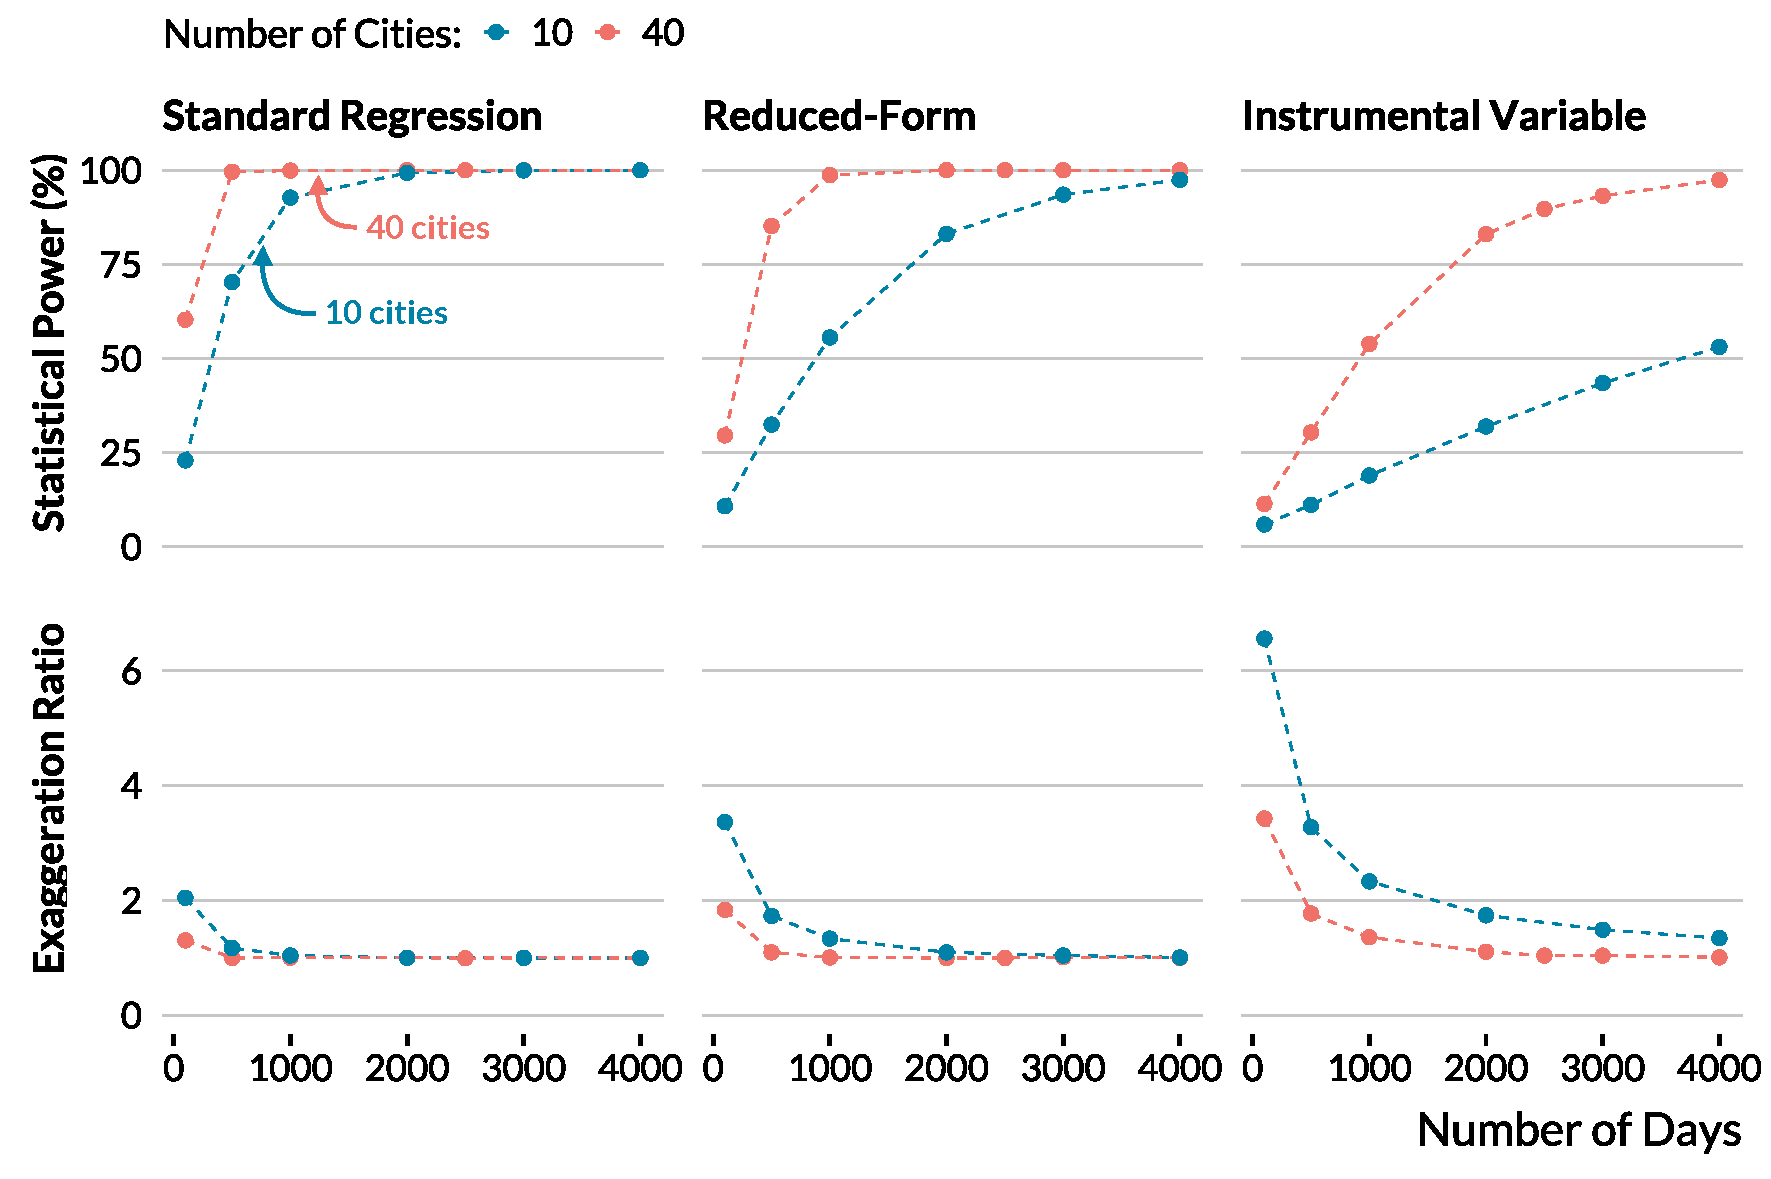
\includegraphics[width=\linewidth]{images/graph_sample_size.pdf}
                \caption*{\footnotesize\textnormal{\textit{Notes}: The other parameters are set to their baseline values: a true effect size of 1\%, 50\% of observations subject to an exogenous shock for instrumental variable and reduced-form designs, and the health outcome is the total number of non-accidental deaths.}}
            \end{figure}
            
            In \Cref{fig:evol_typeM_n_days}, we recover the well-known increasing relationship between the number of observations and statistical power. Conversely, the exaggeration ratio decreases with the number of observations. These results stem from the fact that statistical power decreases and exaggeration increases when the variance of a normally distributed estimator increases \citep{zwet_significance_2021, lu_note_2019} and that the variance of common estimators increases as the number of observations decreases. %For instance, in the homoskedastic case of the OLS, $\hat{\beta} \overset{d}{\to} \mathcal{N}(\beta, \mathbb{E}[\textbf{XX}']^{-1}\sigma^2/n)$, where $n$ is the number of observations, $\hat{\beta}$ the OLS estimate of $\beta$ with standard error $\sigma$, the parameter of interest associated with $\textbf{X}$. 

            We also find that statistical power and exaggeration issues can arise even for a large number of observations. For a sample size of 40,000 observations, the instrumental variable strategy only has a statistical power of 54\% and exaggerates the true effect by a factor of 1.4. On the contrary, the standard regression strategy is much less prone to power issues than the instrumental variable strategy. This is explained by the fact that the variance of the two stage least-square estimator is larger than the variance of the ordinary least square estimator. In our simulations, the probability to make a Type S error is null for all identification methods and sample sizes.
        
        \subsubsection*{Effect Size}
            
            \begin{figure}[ht!]
                \caption{Evolution of Power and Exaggeration with Effect Size.}
                \label{fig:effect_size}
                \centering\includegraphics[width=\linewidth]{images/graph_effect_size.pdf}
                 \caption*{\footnotesize\textnormal{\textit{Notes}: The sample size is 10,000. The other parameters are set to their baseline values: 50\% of observations subject to an exogenous shock for instrumental variable and reduced-form designs, and the health outcome is the total number of non-accidental deaths. For an effect size of 1\%, we do not display the exaggeration ratio of the instrumental variable design since it is above 20 and it would distort the graph.}}
            \end{figure}            
            
            In \Cref{fig:effect_size}, we retrieve another familiar result: the larger the effect size, the larger the power. As expected from \cite{zwet_significance_2021} and \cite{lu_note_2019}'s results, we also find that the exaggeration ratio decreases with the true effect size. Even for our large baseline sample size, statistical power issues appear for effect sizes routinely found in the epidemiology literature. For instance, for our instrumental variable strategy and an effect size of 0.5\%, the average exaggeration ratio is about 1.7. As for results on sample sizes, standard regression and reduced-form strategies are less prone to power issues, even for small effect sizes.
        
        \subsubsection*{Proportion of Exogenous Shocks}
        
            \begin{figure}[ht!]
                \caption{Evolution of Power and Exaggeration with the Proportion of Exogenous Shocks.}
                \label{fig:evol_power_p_treat}
                \centering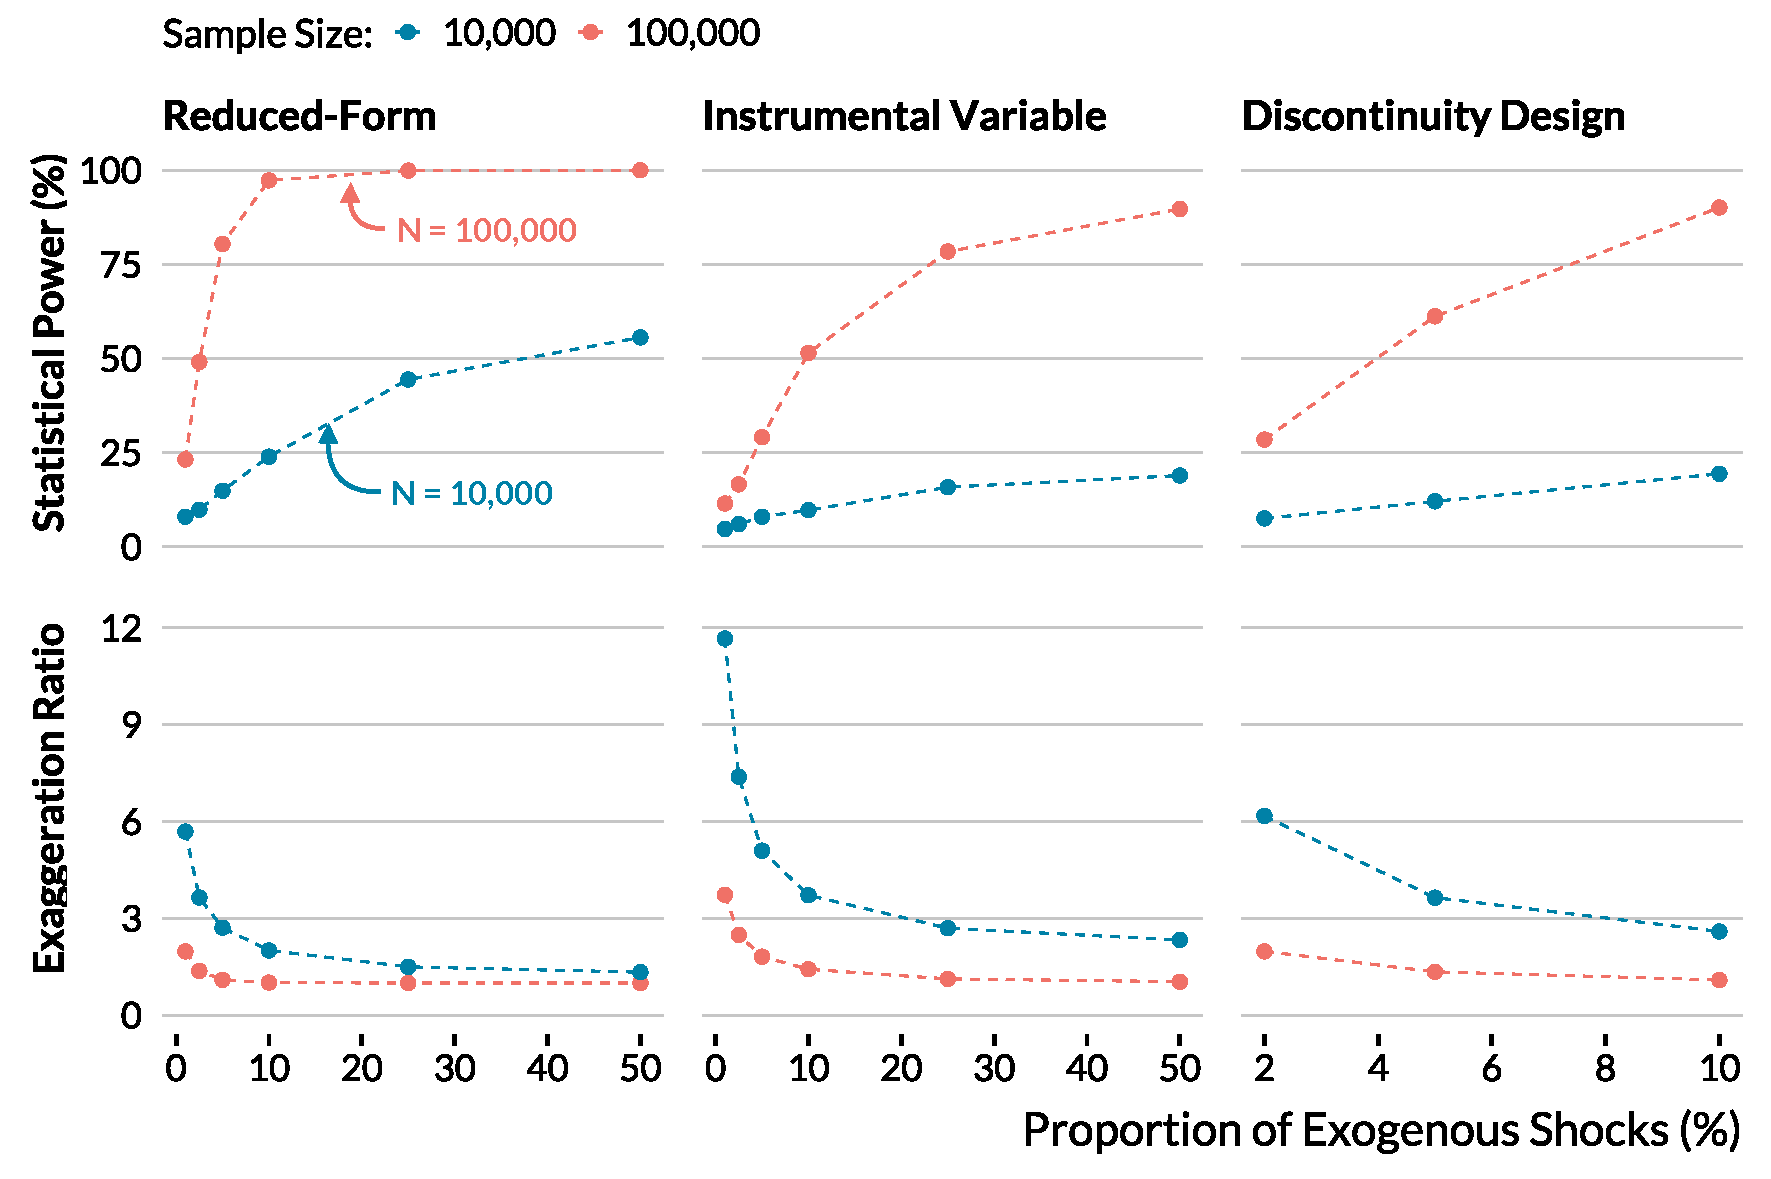
\includegraphics[width=\linewidth]{images/graph_prop_exo_shocks.pdf}
                \caption*{\footnotesize \textnormal{\textit{Notes}: The other parameters are set to their baseline values: a true effect size of 1\% and the health outcome is the total number of non-accidental deaths. The proportion of exogenous shocks corresponds to the fraction of days in the sample that are allocated to the treatment.}}
            \end{figure}
        
            The link between the proportion of exogenous shocks and statistical power might be less widely known. In \Cref{fig:evol_power_p_treat}, we show that statistical power increases with the proportion of treated units for instrumental variable, regression discontinuity and reduced-form designs. Conversely, the average exaggeration ratio increases as the proportion of exogenous shocks decreases. 

            This result can be explained by the fact that exaggeration increases and statistical power decreases with the variance of the estimator \citep{zwet_significance_2021, lu_note_2019}. Now, as routinely discussed for randomized controlled trials but seldom in the case of non-experimental studies, precision is maximized when half of the observations are exposed to the treatment of interest. The variance of the average treatment effect estimator (ATE) is $\sigma^2/[n\times p(1 - p)]$ where $\sigma$ is the standard deviation of the outcome in the treated and control groups and $p$ the proportion of treated units. This quantity increases when $p$ departs from $0.5$. Thus, exaggeration increases when the proportion of exogenous shocks decreases, as long as it was initially smaller than 0.5.
            
            Another way to interpret this result is to consider that a small number of exogenous shocks limits the variation that can be leverage to identify the effect of interest. When the proportion of shocks decreases, the variance of the treatment variable decreases and therefore the variance of the estimator increases. A similar reasoning can be applied to IV strategies.

            \begin{sloppypar}
            In practice, air pollution alerts, thermal inversion or transportation strikes are generally rare events. In some studies, they represent less than 5\% of the observations. With a dataset of 10,000 observations, our simulations return an average exaggeration ratio of 2.7 for the reduced-form strategy. Despite large sample sizes, air pollution studies exploiting few exogenous shocks might be particularly prone to exaggeration issues.
            \end{sloppypar}
            
        \subsubsection*{Average Count of Cases of the Health Outcome}
    
            \begin{table}[!ht]
    \caption{Evolution of Power and Exaggeration with the Average Number of Daily Cases of Health Outcomes.}
    \label{tab:n_cases}
    \centering
            \begin{threeparttable}
                \begin{tabular}{lccc}
                    \toprule
                                         & Non-Accidental & Respiratory & COPD \\ \midrule
                                          %\rowcolor{Gray}
Number of Cases & 23                       & 2                     & 0.3                          \\
Statistical Power (\%)  & 90                       & 16                    & 7.5                          \\
%\rowcolor{Gray}
Exaggeration Ratio      & 1                        & 2.4                   & 5.9                          \\ \bottomrule
                \end{tabular}
                \begin{tablenotes}
                    \footnotesize
                    \item \textit{Notes}: This table displays the average number of cases, the power and the exaggeration ratio for three health outcomes: non-accidental deaths, respiratory deaths, and chronic pulmonary deaths for individuals aged between 65 and 75. These figures are obtained for the instrumental variable design with a sample size of 100,000 and 50\% of observations subject to an exogenous shock. The instrument variable increases the air pollutant concentration by 0.5 standard deviation. A one standard deviation increase in the instrumented air pollutant leads to 1\% relative increase in the health outcome considered.
                \end{tablenotes}
            \end{threeparttable}
\end{table}

            Subgroup analyses are routinely carried out in the literature to evaluate the acute health effects of air pollution on children or the elderly. Yet, the average count of cases can also critically affect statistical power as shown in \Cref{tab:n_cases}. For instance, in a setting with only few deaths per day, a 1\% increase in the number of deaths will rarely cause additional deaths. The effect will be more difficult to detect. To simulate situations with various number of cases, we consider three different outcome variables, with different counts of cases: the total number of non-accidental deaths (daily mean $\simeq$ 23), the total number of respiratory deaths (daily mean $\simeq$ 2) and the number of chronic obstructive pulmonary disease (COPD) cases for individuals aged between 65 and 75 (daily mean $\simeq$ 0.3). Using baseline parameters and in the case of the large dataset, we find that statistical power is close to 100\% for a 1\% increase in the total number of non-accidental deaths. However, statistical power drops when the average count of cases decreases. For instance, the instrumental variable strategy has only 16\% of statistical power to detect a 1\% increase in respiratory deaths. The average exaggeration ratio is then equal to 2.4. For chronic obstructive pulmonary deaths---the health outcome with the lowest number of cases---the situation is even worst since the average exaggeration ratio reaches 5.9. When focusing on subgroups such as children or the elderly, one can expect to find larger effect sizes as those populations are more vulnerable to air pollution. While these larger effect sizes attenuate exaggeration concerns, the lower number of cases exacerbates them. It creates a trade-off for power issues.

        \subsubsection*{Issues Specific to the Instrumental Variable Design}
        
            In the case of instrumental variable strategies, statistical power is affected by the effect size in the first stage of the IV. In our simulations, we consider a binary instrument (e.g., the occurrence of a thermal inversion or a public transport strike). We define its the effect size of the first stage of the IV as the standardized effect size of the instrument on the air pollutant concentration. A IV first stage effect size of 0.2 means that the instrument increases the concentration by 0.2 standard deviation. 
            
            \begin{figure}[ht!]
                \caption{Evolution of Power and Exaggeration with the Strength of the Instrumental Variable.}
                \label{fig:iv_issues}
                \centering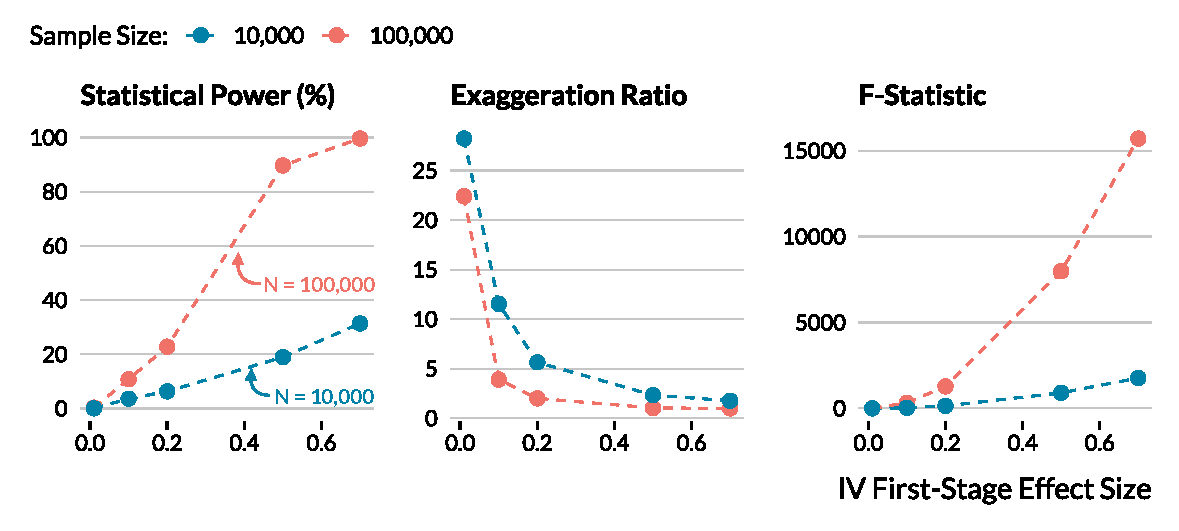
\includegraphics[width=\linewidth]{images/graph_iv.pdf}
                \caption*{\footnotesize \textnormal{\textit{Notes}: The true effect size is a 1\% relative increase in the health outcome. The health outcome used in the simulations is the total number of non-accidental deaths. Half of the observations are exposed to exogenous shocks. The strength of the instrumental variable is defined as its effect in standard deviation on the air pollutant concentration.}}
            \end{figure}
            
            \noindent As shown in \Cref{fig:iv_issues}, we find that statistical power collapses and exaggeration soars when the “IV first stage effect size decreases. Importantly, this issue even arises for large first-stage \textit{F}-statistics. In our simulations based the large data set with 100,000 observations, an instrumental variable's strength of 0.2, and an effect size of 1\%, we find an average \textit{F}-statistics of 1278. The statistical power is however only 23\% and the average exaggeration ratio 2. A large \textit{F}-statistic could therefore hide large exaggeration issues.

            \begin{sloppypar}
            The relationship between IV strength and exaggeration comes from the fact that the variance of the 2SLS estimator decreases with the correlation between the instrument and the instrumented variable. In the homoskedastic case, the asymptotic variance of the 2SLS estimator is $\left(\mathbb{E}[XZ']\mathbb{E}[ZZ']^{-1}\mathbb{E}[ZX']\right)^{-1}\sigma^{2}$, where $\sigma^{2}$ is variance of the error, $X$ the endogenous variable and $Z$ the instrument. When $\mathbb{E}[XZ']$ and $\mathbb{E}[ZX']$ decrease, the variance of the estimator increases. Again, since \cite{zwet_significance_2021} and \cite{lu_note_2019} show that as the variance of a normally distributed estimator increases, the statistical power decreases and exaggeration increases, we obtain the intuition for the simulation results.
            \end{sloppypar}
            
%------------------------------------------------------------------------------

% DISCUSSION

%------------------------------------------------------------------------------

\section{Discussion}\label{section_discussion}

        % why what we did was important
        \begin{sloppypar}
        Growing evidence shows the existence of statistical power issues and publication bias towards statistical significance in economics, causing exaggeration \citep{brodeur_star_2016, ioannidis_power_2017, brodeur_methods_2020, ferraro_feature_2020}. Despite growing awareness of this problem, discussions about the drivers of exaggeration and therefore actionable guidance to tackle it in non-experimental economic research are still lacking \citep{altoe_enhancing_2020, black_simulated_2022}. In this paper, we highlighted a list of concrete drivers of low power and exaggeration we should pay attention to when carrying a non-experimental study. %In the present section, we first discuss the relevance of this list, built based on the example case of studies on the short-term health effects of air pollution, to other contexts. We then propose a principled workflow to assess if and understand why an estimate could be inflated. 
        \end{sloppypar}

        While the simulations we ran were specific to studies on the acute health effect of air pollution, we argue that they can provide lessons for other types of non-experimental studies. First, a large literature investigates the short-term impacts of air pollution on different outcomes such as criminality, cognitive skills and productivity \citep[for instance]{herrnstadt_air_2021, ebenstein_long-run_2016, adhvaryu2022management}. These studies use data with a very similar structure, only focusing on different outcomes and find effects of comparable magnitude or even smaller than those in our literature of interest. Our results should therefore be directly applicable to these literatures. More broadly, settings with typically low signal-to-noise ratios can by definition be subject to power and exaggeration issues. Since as described in \cref{section_results}, the impact of each driver we identified can be explained theoretically, we expect these drivers to affect power and exaggeration in other settings as well. A limited effect size, effective sample size, number of exogenous shocks, average count of the outcome or strength of the instrument can create exaggeration in many settings. Paying careful attention to these factors should help avoid exaggeration issues when running a non-experimental study.
        
        In addition to these specific factors, when carrying out a study, we propose to systematically run retrospective calculations to gauge the risk of exaggeration. They are easy to implement and force us to discuss credible effect size. They allow evaluating if our research design enables us to confidently estimate a credible range of effect sizes. We implemented and discussed such calculations in our literature review and illustrate this approach in more details in Appendix \ref{retro_example} by considering the example of \cite{deryugina_mortality_2019}. As an even simpler first check, we also suggest to consider large confidence intervals verging 0 not only as a sign of uncertainty regarding the exact magnitude of the effect but also of limited power and potential exaggeration of the obtained point estimate.

        Then, we advocate conducting prospective simulations before undertaking a non-experimental study. It allows verifying whether our design can detect effects of a credible magnitude in an almost-ideal setting. Unlike a retrospective analysis, enables us to identify factors that drive exaggeration. Fake-data can be simulated from scratch or simulations can build on datasets used in other studies, as we did in the simulation section of this paper. To facilitate the adoption of this practice, we describe the template we use to run our simulations in the replication material. \cite{black_simulated_2022} also provide useful recommendations to implement power simulations.

        More generally, we advocate paying attention to statistical power in non-experimental studies, even after a statistically significant estimate has been obtained, as insufficient power can lead to exaggeration and inaccurate published estimates. As such, we advocate reporting power calculations to demonstrate the robustness of the design and its ability to accurately capture smaller effect sizes.

        % general recommendations
        On top of these specific comments, we should not forget that published estimates only suffer from exaggeration in the presence of publication bias. In its absence the resulting distribution would be centered around the true effect \citep{hernan_causal_2022}. Adopting a different view towards statistically insignificant results would in particular yield important benefits \citep{ziliak_cult_2008, wasserstein_asa_2016, mcshane_abandon_2019}. To replace the null hypothesis testing framework, we advocate focusing on confidence intervals and to interpret the range of effect sizes supported by the data \citep{amrhein_inferential_2019, romer2020praise}. 
        % final remark
        Qualifying estimates as "statistically significant" does not acknowledge the actual uncertainty that should be computed and embraced to better help policy-makers. Prospective and retrospective power analyses can help design better studies and improve the interpretation of their results.
        
%-----------------------------------------------------------------------------

% BIBLIO

%-----------------------------------------------------------------------------	
        
\singlespacing
\setlength\bibsep{0pt}
\bibliographystyle{aea}
\bibliography{air_pollution.bib}
\onehalfspacing

\pagebreak

%-----------------------------------------------------------------------------

% APPENDIX

%-----------------------------------------------------------------------------	

\appendix

\section{List of Studies Included in the Causal Inference Literature} \label{causal_lit}
\setcounter{figure}{0}
\renewcommand\thefigure{\thesection.\arabic{figure}}   


We display below studies included in the retrospective analysis of the causal inference literature. We group them by research designs:

\singlespacing
\paragraph{Instrumental Variable Design:} \cite{moretti_pollution_2011, ebenstein_particulate_2015, schwartz_estimating_2015, arceo_does_2016, he_effect_2016, knittel_caution_2016, schlenker_airports_2016, sheldon_impact_2017, schwartz_estimating_2017, zhong_traffic_2017, barwick_morbidity_2018, hanlon2018london, schwartz_national_2018, halliday_vog_2019, deryugina_mortality_2019, cheung_mitigating_2020, fan_impact_2020, he_straw_2020, giaccherini_when_2021, godzinski_disentangling_2021, guidetti_placebo_2021, kim_air_2021, liu_effect_2021, xia_short-term_2022}

\paragraph{Reduced-Form Design:} \cite{bauernschuster_when_2017, jans_economic_2018, jia_is_2019, godzinski2019short}

\begin{sloppypar}
\paragraph{Regression Discontinuity Design:} \cite{chen_air_2018, fan_winter_2020, anderson2022bounds}


\paragraph{Event-Study Design:} \cite{mullins_effects_2015, simeonova_congestion_2021}
\end{sloppypar}

\paragraph{Matching Design:} \cite{baccini_assessing_2017, forastiere_assessing_2020}
\onehalfspacing


\section{Implementing a Retrospective Power Analysis} \label{retro_example}

We explain here how we can easily implement a retrospective power analysis once a study is completed. In a flagship publication, \cite{deryugina_mortality_2019} instrument PM$_{2.5}$ concentrations with wind directions to estimate its effect on mortality, health care use, and medical costs among the US elderly. They gathered 1,980,549 daily observations at the county-level over the 1999–2013 period; it is one of the biggest sample sizes in the literature. When the authors instrument PM$_{2.5}$ with wind direction, they find that “a 1 $\mu \text{g/m}^3$ (about 10 percent of the mean) increase in PM$_{2.5}$ exposure for one day causes 0.69 additional deaths per million elderly individuals over the three-day window that spans the day of the increase and the following two days”. The estimate's standard error is equal to 0.061. In \Cref{fig:deryugina}, we plot the statistical power, the inflation factor of statistically significant estimates and the probability that they are of the wrong sign as a function of hypothetical true effect sizes.
    
        \begin{figure}[!ht]
            \caption{Power, Type M and S Errors Curves for \cite{deryugina_mortality_2019}.}
            \label{fig:deryugina}
        \centering\includegraphics[width=\linewidth]{images/iv_example.pdf}
            \caption*{\footnotesize \textnormal{\textit{Notes}: In each panel, a metric, such as the statistical power, the exaggeration ratio or the probability to make a type S error, is plotted against the range of hypothetical effect sizes. The "IV" label represents the value of the corresponding metric for an effect size equal to \cite{deryugina_mortality_2019}'s two-stage least square estimate. The "Epidemiology" label stands for the estimate found in \cite{di_association_2017}, which is the epidemiology article most similar to \cite{deryugina_mortality_2019}. The " Naive OLS" label corresponds to the estimate found by \cite{deryugina_mortality_2019} when the air pollutant is not instrumented.}}
        \end{figure}
    
    The estimate found by \cite{deryugina_mortality_2019} represents a relative increase of 0.18\% in mortality. We labeled it as "IV" in \Cref{fig:deryugina}. Is this estimated effect size large compared to those reported in the standard epidemiology literature? We found a similar article to draw a comparison. Using a case-crossover design and conditional logistic regression, \cite{di_association_2017} find that a 1 $\mu \text{g/m}^3$ increase in PM$_{2.5}$ is associated with a 0.105\% relative increase in all-cause mortality in the Medicare population from 2000 to 2012. The effect size found by \cite{deryugina_mortality_2019} is larger than this estimate labeled as "Epidemiology" in \Cref{fig:deryugina}. If the estimate found by \cite{di_association_2017} was actually the true effect size of PM$_{2.5}$ on elderly mortality, the study of \cite{deryugina_mortality_2019} would have enough statistical power to perfectly avoid type M and S errors. Now, suppose that the true effect of the increase in PM$_{2.5}$ was 0.095 additional deaths per million elderly individuals---the estimate the authors found with a "naive" multivariate regression model. The statistical power would be 34\%, the probability to make a type S error could be null but the exaggeration factor would be on average equal to 1.7. Even with a sample size of nearly 2 million observations, \cite{deryugina_mortality_2019} could make a non-negligible type M error if the true effect size was the naive ordinary least square estimate. Yet, the authors could argue that their instrumental variable strategy leads to a higher effect size as it overcomes unmeasured counfounding bias and measurement error. Besides, for effect sizes down to 0.182 additional deaths per million elderly individuals (a 0.05\% relative increase), their study has a very high statistical power and would not run into substantial type M error. A retrospective analysis is thus a very convenient way to think about the statistical power of a study to accurately detect alternative effect sizes.

    \section{Case Studies}  \label{case_studies}

        The main simulation results help understand how the various parameters influence the statistical power of studies. Yet, these parameters may not perfectly represent actual studies as we made several conservative assumptions: relatively large sample size, proportion of treated units, average outcome counts and instrumental variable strength. For each research design, we therefore consider a realistic set of parameters based on an example from the literature. We then vary the value of key parameters. As we are working with different data, we cannot exactly reproduce the level of precision found in the articles considered. Our goal is not to claim that the estimates produced by a particular article are inflated, but instead to understand how low power issues could arise for representative parameter values.
            
        \subsection*{Public Transportation Strikes}
        
            Public transportation strikes are unique but rare positive shocks to air pollution as individuals use their cars to reach city centers. Even in a large data set, with several cities and a long study period, the proportion of affected days might be very small. For instance, \cite{bauernschuster_when_2017} investigate the effect of public transportation strikes on air pollution and emergency admission in the five biggest German cities over a period of 6 years. Despite a sample size of 11,000, there are only 57 1-day strikes during the study period (0.5\% of days are actually treated). The authors find that children hospitalizations for breathing issues increase by 34\% (SE=8\%) on strike days. On average, 0.22 children per day go to the hospital for breathing issues.
            
            We simulate a similar design with our own data. We first randomly sample 2200 observations for five cities and then vary (i) the proportion of exogenous shocks from 0.5\% up to 10\%, and (ii) the treatment effect size from a 4\% increase up to a 34\% increase. We focus on elderly mortality due to chronic obstructive pulmonary disease since it has an average daily count of 0.29 cases. 
            
            
            \begin{figure}[ht!]
                \caption{Evolution of Power and Exaggeration for Public Transportation Strikes Designs.}
                \label{fig:strikes}
                \centering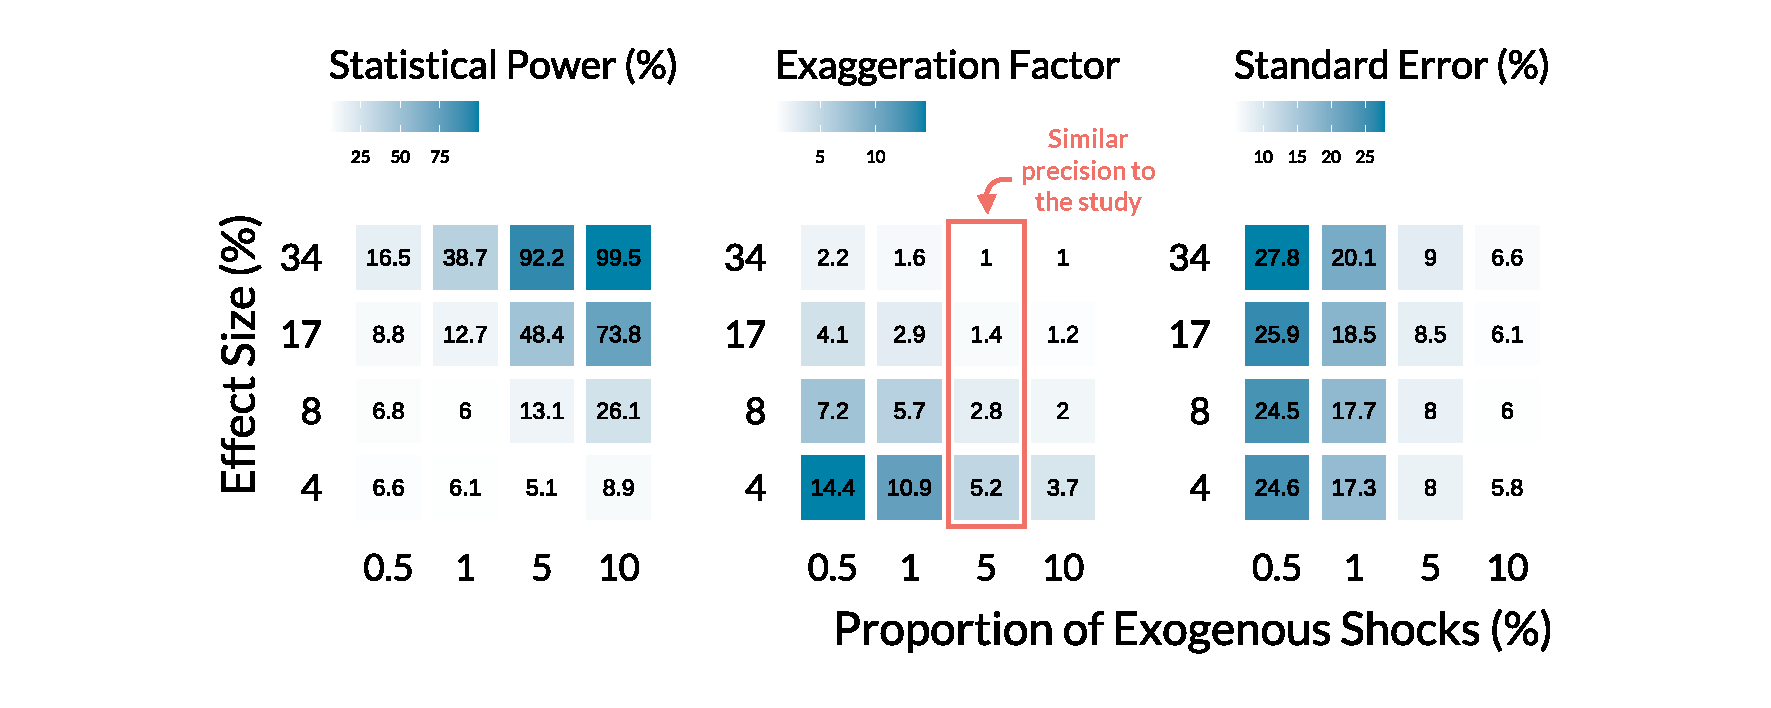
\includegraphics[width=\linewidth]{images/graph_strikes.pdf}
                \caption*{\footnotesize \textnormal{\textit{Notes}: Each panel displays the average value of a metric (power, exaggeration, and standard error) for varying proportions of exogenous shocks and effect sizes. The average standard error of simulations is the raw standard error divided by the mean number of cases of the health outcome. For each combination of parameters, we ran 1000 simulations.}}
            \end{figure}
            
            In \Cref{fig:strikes}, we display our simulation results. The first panel from the left shows that both large effect sizes and a large proportion of exogenous shocks are required to reach adequate power. In the middle panel, we show that a proportion of 0.5\% of exogenous shocks is associated with very large exaggeration ratios, from 2.2 for a true effect size of 34\% up to 14 for one of 4\%. Power issues fade for a combination of a proportion of exogenous shocks above 5\% and effect sizes above 17\%. In the right panel, we plot the average standard error of the estimates, expressed as a fraction of the average of the health outcome. The standard error of \cite{bauernschuster_when_2017}'s is 8\%. In our simulations, we recover that specific precision for a proportion of exogenous shocks of 5\%. In that case, a true effect size of 34\% would not yield inflated estimates. However, if effect sizes are actually smaller and more representative of those found in the literature, the exaggeration would be consequential.
            
            This simulation exercise shows that exaggeration is likely to arise in practice since the proportion of exogenous shocks is low. It occurs even when true effect sizes are relatively large.
        
        \subsection*{Air Pollution Alerts}
            
            Air pollution alerts are also rare events. Their effects are estimated using regression discontinuity designs that restrict the analysis to observations closed to the air quality threshold. As a consequence, the effective sample size may be particularly small. For instance, \cite{chen_effect_2018} investigate the effects of air quality alerts on emergency department visits in Torento, over the 2003-2012 period. While the nominal sample size is 3652, the effective one is only 143 (100 control days and 43 treated days). Only 1.2\% of observations are treated. The authors find that eligibility to air quality (the intention-to-treat effect) approximately reduces emergency visits for asthma by 8\% (SE=3.8\%). The average daily count of cases of their health outcome is 26.
        
            We approximate the setting of \cite{chen_effect_2018} using our data. We first sample one city for a time period of 3652 days and randomly allocate the treatment. We then repeat the process varying the proportion of alerts and effect sizes. Our outcome variable is the total number of non-accidental deaths since it has a daily mean of 23.
            
            \begin{figure}[ht!]
                \caption{Evolution of Power and Exaggeration for Air Quality Alerts Designs.}
                \label{fig:alerts}
                \centering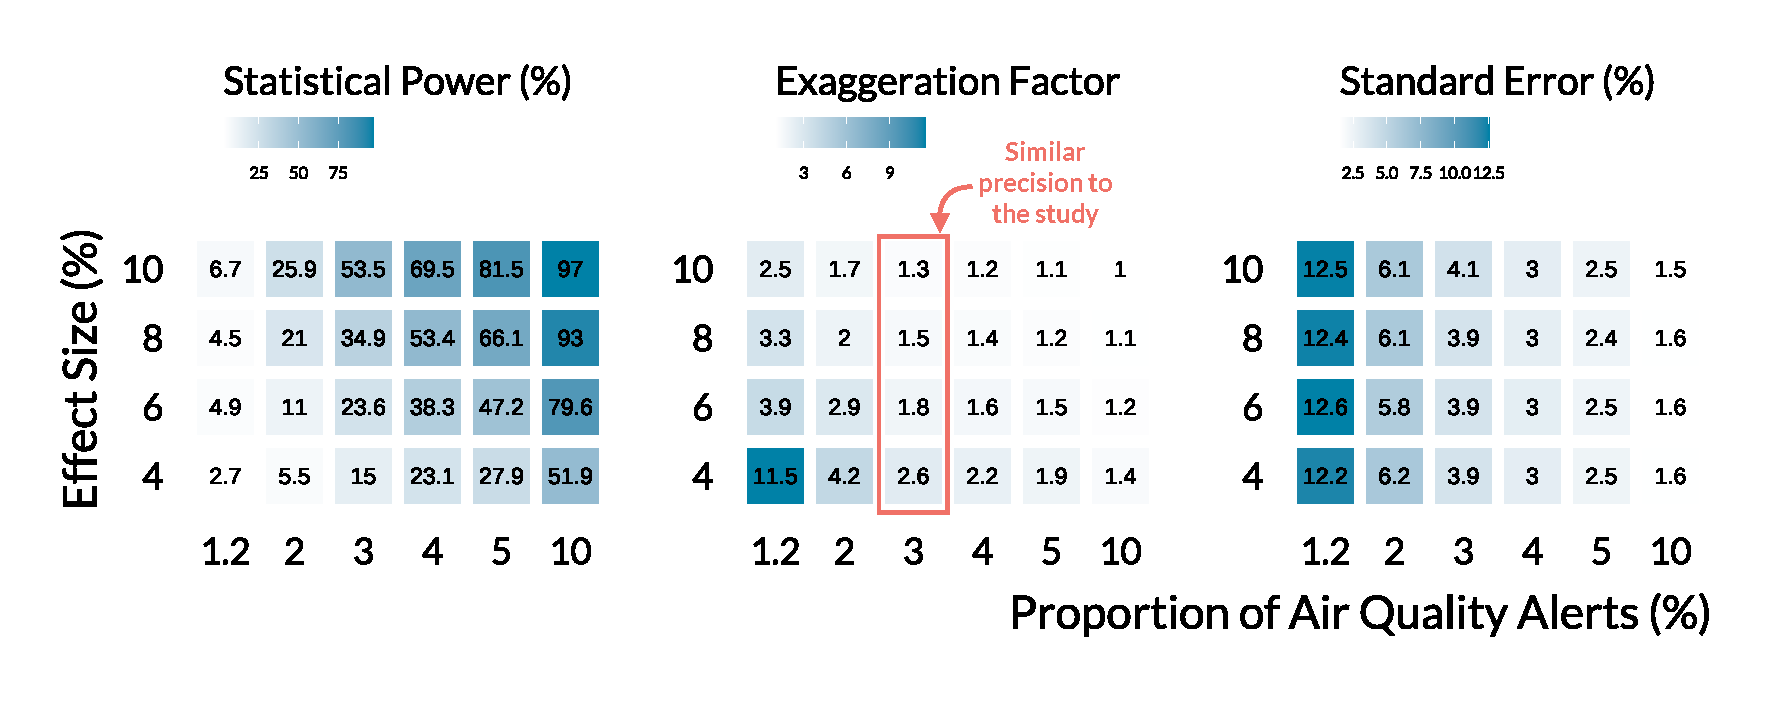
\includegraphics[width=\linewidth]{images/graph_air_quality_alerts.pdf}
                \caption*{\footnotesize \textnormal{\textit{Notes}: Each panel display the average value of a metric (power, exaggeration, and standard error) for varying proportions of exogenous shocks and effect sizes. The average standard error of simulations is the raw standard error divided by the mean number of cases of the health outcome. For each combination of parameters, we ran 1000 simulations.}}
            \end{figure}   
            
            \Cref{fig:alerts} displays the simulations results. As in \Cref{fig:strikes}, a combination of large effect sizes and many air quality alerts is needed to avoid low power issues. We get a precision similar to \cite{chen_effect_2018} for a proportion of air quality alerts of 3\%. For an effect size of 4\%, the average exaggeration ratio is equal to 2.6. In that case, the average average of statistically significant estimates is 10\%, which is similar to the effect size found by \cite{chen_air_2018}.
            
            Unless true effect sizes are very large, air quality alert designs produce inflated estimates in realistic settings.
        
        \subsection*{Instrumenting Air Pollution}
        
            Finally, we investigate the most commonly used strategy in the causal inference literature, the instrumental variable design. Several studies rely on very large datasets and exploit changes in weather patterns as sources of exogenous variations. For instance, \cite{schwartz_national_2018} instrument PM$_{2.5}$ concentration with planetary boundary layer, winds speed, and air pressure. Once the effects of seasonal and other weather parameters are accounted for, the combination of their instruments explains 18\% of the variation in PM$_{2.5}$ concentration. They find that a 10 $\mu \text{g/m}^3$ increase in PM$_{2.5}$ leads to a 1.5\% (SE=0.22\%) increase in daily non-accidental mortality. There are on average 23 daily deaths in their dataset of 591,570 observations (135 cities with a length of study of approximately 4382 days).
            
            In our simulations, we assess how the strength of the instrumental variable affects power issues for several health outcomes. We consider a binary instrumental variable and vary its effect on air pollution concentration from a 0.1 to a 0.5 standard deviation increase. The 18\% correlation in \cite{schwartz_national_2018} corresponds to a 0.4 standard deviation increase in our case \citep{lipsey2001practical}. We assume that half of the observations are exposed to exogenous shocks. We set an effect size corresponding to a 1.5\% relative increase in three health outcomes with different average number of cases: non-accidental mortality (mean cases of 23), respiratory mortality (mean of 2), and chronic obstructive pulmonary mortality of elderly (mean of 0.3). Our data set being smaller than the one used in \cite{schwartz_national_2018}, we only run simulations for a sample size of 100,000.
        
            \begin{figure}[ht!]
                \caption{Evolution of Power and Exaggeration for Instrumental Variable Designs.}
                \label{fig:iv_wind}
                \centering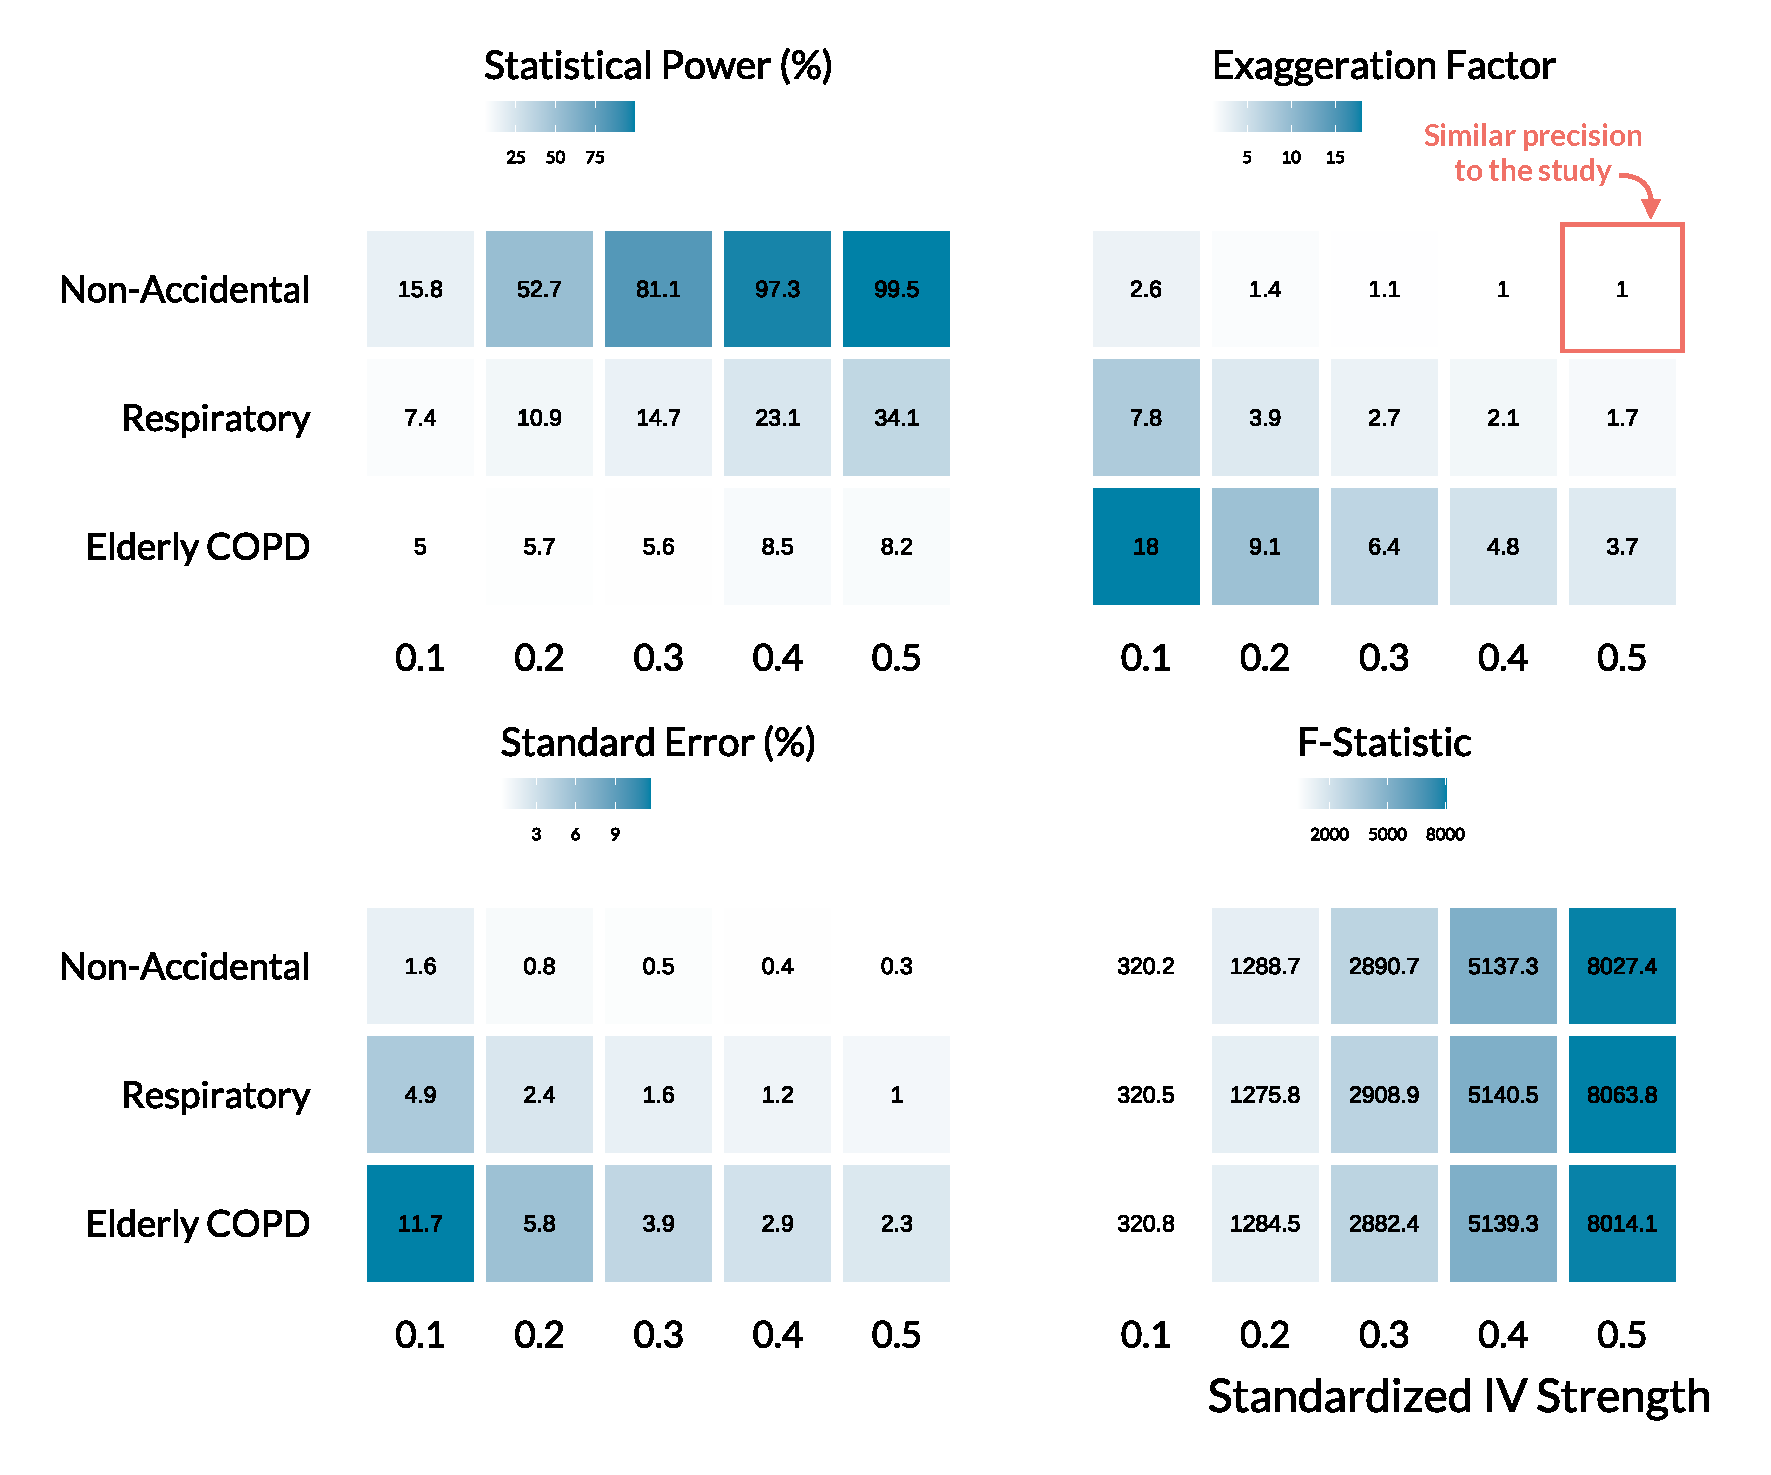
\includegraphics[width=\linewidth]{images/graph_iv_wind.pdf}
                \caption*{\footnotesize \textnormal{\textit{Notes}: Each panel display the average value of a metric (power, exaggeration, standard error, and first-stage \textit{F}-statistic.) for varying proportions of exogenous shocks and effect sizes. The average standard error of simulations is the raw standard error divided by the mean number of cases of the health outcome. For each combination of parameters, we ran 1000 simulations.}}
            \end{figure} 
            
            In \Cref{fig:iv_wind}, we see in the top-left panel that power reaches satisfactory level for large instrumental variable strengths but only for non-accidental causes. For respiratory and elderly mortality, exaggeration can be substantial even for large IV strength. While our sample size is large, it is smaller than the one in \cite{schwartz_national_2018}. As a consequence, our simulations only have a precision close to theirs for an instrumental variable strength of 0.5 and non-accidental mortality. Yet, our simulations highlight that important exaggeration issues can arise in realistic settings, even for large IV strength. The bottom-right panel of \Cref{fig:iv_wind} confirms the result found in the simulations of the previous section: a large first stage \textit{F}-statistic can be a poor indicator of statistical power issues. For instance, for non-accidental mortality and an IV strength of 0.1, the \textit{F}-statistic is equal to 320 but the exaggeration factor is 2.6, with an associated estimated power of 16\%. Importantly, as the \textit{F}-statistic does not vary with the number of cases in the outcome it can all the more hide important power issues.
            
                    
\end{document}
 